        
        \section{Cosmic sources of gravitational waves}
        \label{cosmic_sources}
      
        %   --- Cosmic origins believed to generate GW. (note: should sprinkle citations as needed, not just where it says "cite") ---

		Gravity's power to induce ripples in space is a matter of fact. Pulsar 1913+16, discovered by Hulse and Taylor in radio waves, not only followed a pattern of orbital decay consistent with radiative loss of orbital decay to gravitational radiation -- it continued to do so~\cite{WeisbergTaylor2004,Weisberg2010}, seen in Figure~\ref{Hulse-Taylor_binary}, after the 1993 physics Nobel Prize. 
This year, there has been much debate whether the BICEP2~\cite{BICEP2014} and Planck~\cite{Planck2014} probes of the cosmic microwave background have seen evidence of $B$-mode polarizations that would indicate primordial gravitational fluctuations.
Eventual identification of the polarization is expected regardless. 
We still may ask whether any gravitational waves will be directly detectable on Earth. 
We may ask whether they appear in detectors in a way consistent with general relativity. 
The basic fact of their emission, however, appears settled.

	\begin{figure}
	\begin{center}
	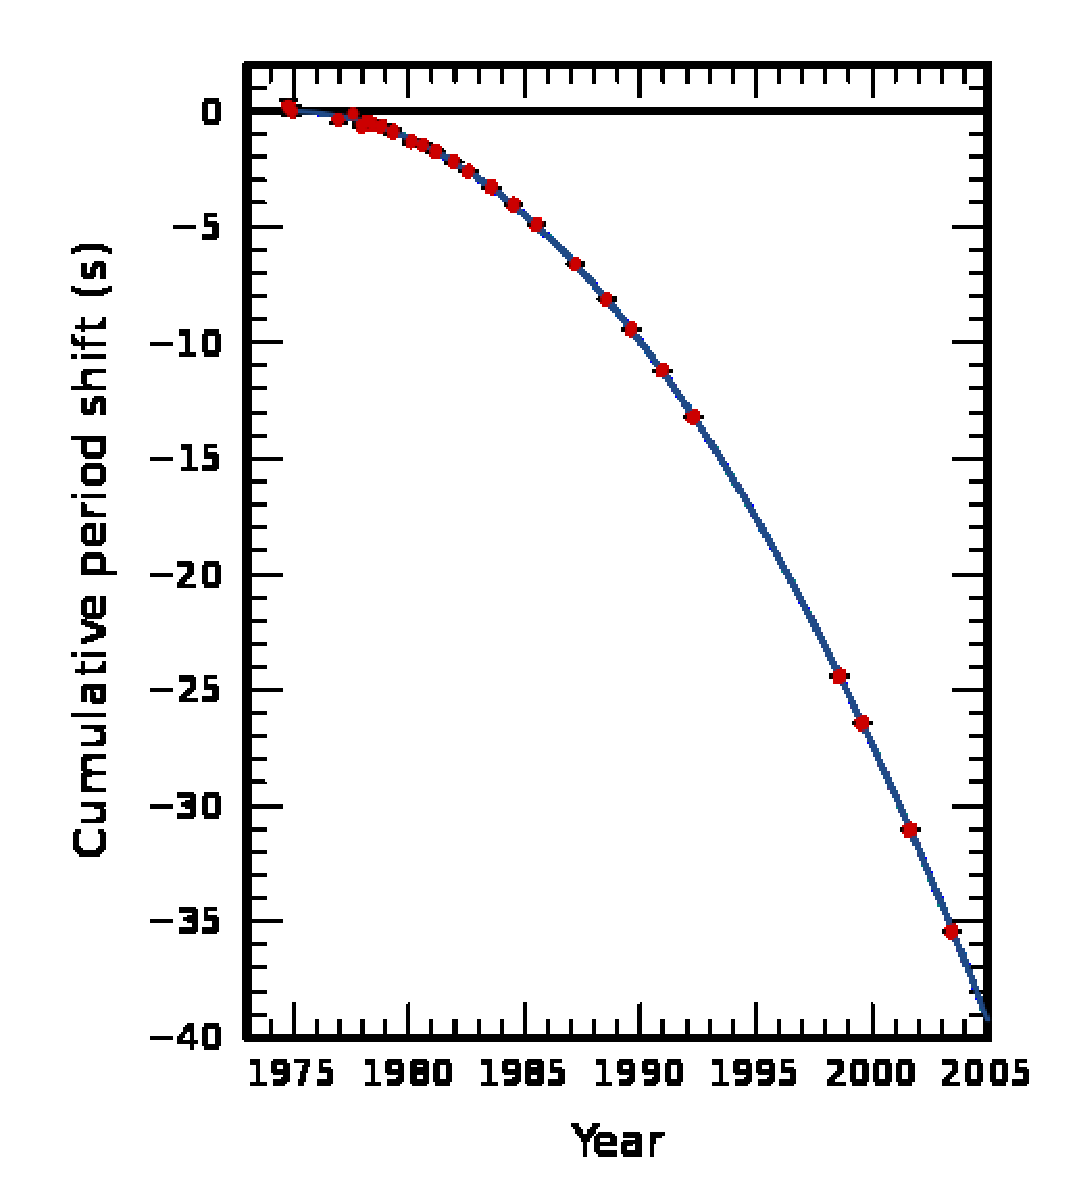
\includegraphics[height=111mm, width=148mm]{500px-PSR_B1913+16_period_shift_graph.eps}
	\caption{The Hulse-Taylor binary PSR 1913+16, orbital period change over time consistent with emission of gravitational radiation from its system~\cite{Weisberg2010}. Gravitational waves emission depletes orbital energy, causing the binary stars to slowly inspiral into closer orbits. Shrinking pulsar radius $R$ leads to the shorter period $T$ -- Kepler's third law, $T \propto R^{3/2}$ (first stated in \textit{Harmonices Mundi}~\cite{Hawking2002}). Timing error can be ruled out, because the orbital decay is not linear.}
	\label{Hulse-Taylor_binary}
	\end{center}
	\end{figure}

Before delving into general relativitic emission, let us consider the astrophysical sources expected to emit gravitational waves. 
Physics prompts our search, but astronomy makes it exciting.
When gravitational waves are heard by the interferometers, the public should remember them as the songs of dead stars, rippling through the fabric of spacetime.  
Gravitational waves (henceforth also abbreviated GW) searches presently focus on four distinct types of cosmic sources.
This categorization of sources was presented no later than the 1983 LIGO Blue Book proposal and has since guided research focus~\cite{CollinsGravityShadow,Schutz1989}. 
The quadripartite division:
\begin{itemize}
\item Burst (rarely, `supernova')
\item Compact binary coalescence (or `inspiral')
\item Continuous wave (or `pulsar')
\item Stochastic
\end{itemize}

This thesis concentrates on continuous waves (CW) -- sine waves. 
CW are most likely to emanate from neutron stars. 
Perhaps neutron star CW modulated by orbital motion, spun-up from accretion or spun-down from radiated energy. 
Given a sufficiently large ellipticity, on the order of $\epsilon \approx 10^{-7}$~\cite{Owen2005} or smaller for a neutron star rotating on the order of 1 kHz, a crust deformation (perhaps due to an $r$-mode) would radiate sufficient gravitational radiation to be a plausibly-detectable source. 
Indeed, the radiation would rapidly deplete the rotational energy of the neutron star~\cite{Owen1998}, which is why binary systems, where the neutron star could be recycled and spun-up by a partner, prove a promising target~\cite{PapaloizouPringle1978,Wagoner1984}. 
Scorpius X-1 offers a canonical case~\cite{AbbottScoX12007}, although the TwoSpect search anticipates an abundance of other low-mass X-ray binary (LMXB) systems of interest. 
Given the paucity of insight on the interiors of collapsed stellar remnants, direct detection of GW from neutron stars would prove informative. 
Just as we might infer details from neutron star binary coalescences favoring one equation of state~\cite{Lattimer2007,Read2009}, we might also extract parameters from continuous waves suggesting the existence of quark stars or gravitars~\cite{Owen2005}, and will have an unparalleled peek into the interior of the densest stable three-dimensional objects in the universe. 
Their simple waveforms might even facilitate the calibration of other types of GW data, whereas binary mergers should sound like standard sirens to compare against electromagnetic and neutrino observations~\cite{Punturo2010}
(see next paragraph).
CW are conceptually-elegant and astronomically-enticing.
Yet other sources of GW have a comparable pull on our attention. 

Inspirals or compact binary coalescences occur when two stellar remnants draw nearer in their orbits, radiating gravitational radiation and finally merging in a titanic release of energy. 
While sometimes invisible -- the merging of black holes in short-hard gamma ray burts (GRBs) being an exception -- these events compete eagerly with supernovae as the most explosive in the modern universe. 
Were GW observatories to see their waveforms, they could be compared with those predicted through post-Newtonian approximation and numerical relativity. 
As GW amplitude should diminish linearly with distance, we would then have standard candles or \textit{standard sirens} by which to calibrate and measure the universe. 
Advanced LIGO~\cite{aLIGOrefDesign,aLIGOsysDesign} may prove sensitive to neutron star-neutron star and stellar mass black hole-neutron star mergers, and, if low-frequency sensitivity is sufficient and the sources exist, to intermediate-mass black holes. 
Space-based observatories such as the longsuffering Laser Interferometer Space Antenna (LISA) and ensuing DeciHertz Gravitational-wave Observatory (DECIGO) \& Big Bang Observer (BBO) could detect supermassive black hole mergers. If launched, they would see a low-frequency noise floor due not to seismic vibration, as in LIGO, but to white dwarf binaries throughout the galaxy. 
Since the waveforms are well-predicted, we could even investigate deviations from general relativity, perhaps seeing new physics in the ringdown of black holes.

Physical insight could also come from burst searches. 
Bursts share with inspiral searches the property of looking for a single event, as opposed to a source spread over long duration. 
Analytical programs for bursts can sometimes be applied to inspiral or detector characterization tasks as well; rare noise events are a limit on their astronomical sensitivity.
Yet the immediate focus lies with supernovae and perhaps gamma-ray bursts. 
Because the waveform is unknown, burst searches rely significantly more on the coincidence between multiple detectors to distinguish signal from noise. 
Just as with neutrino observations of supernova 1987A, the burst program would hope for a fortuitously nearby cataclysm to be seen simultaneously -- or nearly so, the time of flight indicating a direction -- in a global gravitational-wave detector network. 
Due to the versatility of this method, some researchers have proposed looking for longitudinal polarization in addition to plus and cross orthogonal polarization (possible in non-general relativistic terms; see Section~\ref{history_GR}). 
Any detection would be quite exciting for probing systems still mysterious with electromagnetic and neutrino measurements, and it would help, in conjunction with multi-messenger coordinated searches with those observatories, to ascertain at precisely what speed gravity travels through space-time and to what extent it is attenuated or altered.

The background of space-time itself may hide GW signatures. 
Searches for the stochastic GW background look not for single events but for persistent phenomena buried in many months of correlated signals between networks of detectors. 
In doing so, they hope in particular to see the earliest turbulence of the universe -- long before the cosmic electromagnetic background, now microwaves, was emitted 380000 years after the Big Bang, GW were travelling unimpeded. 
While the opacity of the infant cosmos conflates electromagnetic signals from different times and places, the transparency of the universe to gravity means that we might see the inflationary epoch or earlier, the Planck time. 
Unfortunately, this signal is thought to be far below the sensitivity of existing detectors. 
While LIGO did set a new upper limit on the energy density of GW, measured as a fraction, $\Omega_{gw}$ of the critical closure density of the universe~\cite{LIGOStochasticNature2009}, the inflationary background at LIGO frequencies is predicted to be about ten orders of magnitude lower. 
Alternative theories, such as ekpyrotic/cyclic universes, make other predictions, so an anomalously high stochastic background could prove cosmologically significant.

All GW searches would open up new directions in astronomy. 
While the most exciting possibility is that we will see the unexpected, we think that our present algorithms will permit serendipity while efficiently categorizing computational challenges. 
Continuous wave and inspiral methods both search against waveform templates; burst and stochastic have no template and rely on correlation and coincidence. 
Continuous wave and stochastic analyze weeks, months, even years of data in search of persistant features; inspiral and burst look for transient events. 
In the abstract dimensions of search groups, we are complete. 
Our blind spots are in what data we provide to those groups -- in the focus on audio frequencies of tens to a few thousand Hertz at present -- blindness that will in time be rectified by CMB polarization, pulsar-timing and space-based interferometry for low frequencies and possibly by atom interferometry for high frequencies. 
To appreciate our choice of focus in these nascent days of the field, we must turn back a century to understand its origins in Einstein's mathematics.

        \subsection{History from general relativity}
        \label{history_GR}

            %Historical brief of Einstein.
        Einstein's theory unified a sequence of historical insights. 
Since 1676, when Roemer used the moons of Jupiter to measure the finite speed of light, just before Newton's 1687 \textit{Principia Mathematica}~\cite{Hawking2002}, the question of gravity's propogation beckoned. 
Bringing together the work of Minkowski and Poincar\'{e}, the 1905 special theory of relativity highlighted the naturalness of the speed of light, but only in 1915, with the presentation of the Einstein field equations of general relativity, based in Riemannian geometry, did a means to an answer emerge. 
In 1916, Einstein predicted GW. 
At last, gravity had a theoretical speed: the same as that of electromagnetism, that of light in the vacuum, $c$.
In the linear approximation to the nonlinear theory of general relativity (henceforth GR), the waves were mathematically similar to the waves of electromagnetism, as will be shown in Section~\ref{general_relativity}.
GR offers a consistent explanation for how changes in the distribution of matter change gravitational fields.
Yet the detectability of the waves, even in principle, would remain an open question for another half century. 
Uncertainty in whether fluctuations within spacetime could be detectable with instruments themselves changed by the fluctuations dominated the debate.
Consult Misner, Thorne, and Wheeler's \textit{Gravitation}~\cite{MisnerThorneWheeler} and Sean Carroll's lectures notes~\cite{Carroll1997}, as well as other history books of the field for an account of the controversy.
Thought notions, \textit{Gedankenexperiment}, such as beads-on-rods led to consensus that GW carried and could deposit physical energy and thus be detected. 
See \textit{Gravity's Shadow}~\cite{CollinsGravityShadow} for sociological perspective, and 
\textit{Gravity's Ghost}~\cite{CollinsGravityGhost} for insight into the detection criteria that have since evolved\footnote{See also a recent review by Riles~\cite{Riles2013}.}.

Discussions of GW frequently begin with derivations of the wave equations from Einstein's field equations. 
General relativity, however, is not the only theory to predict GW: waves are a natural consequence of a class of similar theories, which make a range of testable predictions (such as number of polarization modes, from two to six, and possibly speeds different from $c$)~\cite{Will1993}. 
Waves should thus be expected even if some minor variation from Einstein's theory is discovered, pointing a way perhaps toward a quantum theory of gravity~\cite{Sathyaprakash2009}. 
%As the field progresses toward first detection and beyond to astronomy, the astrophysical targets of our searches should take precedence.

Before deriving the answer to the detectability question from the field equations, a contrast with the situation in other fields of astronomy is in order.

 
        \subsection{Contrast with electromagnetic and particle astronomy}
        \label{contrast_astro}

        With astronomy, detection came first, then theory.
Visible light astronomy began with the earliest humans.
Records of the star Sirius are known from Egyptian astronomers, the planet Venus from Babylonians, sunspots from the Chinese, and eclipses from the Greeks. 
Thus the telescope, though revolutionary, was not unimaginable.

Infrared radiation, as first seen by William Herschel, was just beyond the visible red light of a prism.
As the wave nature of light came to be understood, culminating in Maxwell's equations, the existence of invisible electromagnetic radiation was put on sound theoretical footing.
The only remaining questions pertained to whether this radiation would prove astornomically interesting, especially in the extreme low- (radio) and high- (X- and $\gamma$-ray) frequencies found at the end of the 19th Century.
Fortuitiously, unlike with GW today, these novel bands of electromagnetic spectrum could be easily generated and detected by scientists in small laboratories, as with Marconi and Marie \& Pierre Curie.
Within half a century, radio telescopy began with Karl Jansky~\cite{Shklovsky1960}, with Grote Reber soon observing the Milky Way~\cite{Gurzadyan1956}.
By the early 21st Century, radio astronomy ranged from common rooftop designs~\cite{SRT} (nonetheless sensitive enough to infer the galactic rotation curve in the hydrogen line~\cite{MeadorsThesis2008}) to planetary-scale very long baseline interferometry and plans for a Square Kilometer Array.
Electromagnetic, or photon, astronomy has the advantage of calibration with familiar sources.

%            Contrast with electromagnetism, compare with radio/X-ray/et cetera astro. 

%Can make analogy to radio waves and make note of the ease with which one can operate a small radio telescope, as I did in my thesis~\cite{MeadorsThesis2008}, compared the the difficulty of GW detection. 

Other particles besides the photon began to play a role in 20th Century astronomy.
Muons from space were detected long ago, as in C.D. Anderson's 1949 paper on what was then called the mesotron~\cite{CDAnderson}. 
Solar neutrinos were, after much difficulty, seen by John Bahcall~\cite{NeutrinoReview}, and neutrino astronomy is a well-established field by the turn of the millenium, following the detection of Supernova 1987A in the Large Magellenic Cloud. 
New types of neutrino detectors (for example, time-projection chambers~\cite{EBubble2005,MeadorsNevis2006}) could yield additional information and better sensitivity, but as with electromagnetism, the calibration question is resolved. 
Since the Savannah River nuclear reactor experiments, the experimental detectability of neutrinos has been settled, and though the 1964 theory of solar neutrinos~\cite{NeutrinosSolarTheoretical} required tuning to account for neutrino oscillation, astrophysics with neutrino observatories is becoming mature.
Nuclear fusion in the Sun has been well-established, and arrays such as Antares and IceCube will move the field outwards toward cosmic sources.


 GW from the PSR 1913+16 pulsar itself~\cite{WeisbergTaylor2004} are too low in frequency to be seen with existing interferometers, but they confirm that the phenomena is real.
Although no terrestrial sources of GW can be feasibly generated, calibration~\cite{AbadieCalibration2010} of interferometers is nonetheless accurate to a few percent.
Direct detection of GW would let us infer the true strength of astrophysical gravitational radiation and compare that power with theory. 
Surprising new insights are probable in any new field, not unlike the discovery of neutrino oscillation in the solar spectrum or the anomalous galactic rotation curve due to dark matter, are probable in any new field.

Yet how can gravity been seen?
GW are conceptually simple, with mathematics illustrated by electrodynamic analogy in the Appendix.
A short derivation follows.

    %End section by very rapidly deriving wave equation of electricity and magnetism, to lead by example for how we go about GR.
    %Note that all physics in min(action),
    %introduce metric as inner product
    %generally, coordinate transform good



    \section{General relativity}
    \label{general_relativity}

        Einstein's theory of General Relativity (hence GR) describes gravitation as curvature. 
Gravity is a pseudoforce, unlike Newton's force $\textbf{F} = -G_C M_1 M_2 r^{-2} \hat{\textbf{r}}$ for two bodies of masses $M_1$ and $M_2$ seperated by a vector distance $\textbf{r}$ in a universe with a gravitational constant $G_C$ (henceforth, units are set where $G_C \equiv 1$).
 Einstein posits that objects always follow an extremized path, $\delta s = 0$ for arclength $s$  -- a geodesic worldline -- when the curvature of spacetime is considered. 

The curvature of spacetime is described by the Riemann tensor, $R^\mu_{\nu\rho\sigma}$, which physically is required to be a solution to the Einstein field equations. 
Section~\ref{field_equations} clarifies the connection between these field equations and the Ricci scalar curvature $R$, a trace of the Riemann tensor, whence they can be derived. 
This Riemann tensor is constructed from the Christoffel connection, $\Gamma^\mu_{\rho\sigma}$, which in turn can be expressed in terms of the metric, $g_{\mu \nu}$.
It is the metric that measures distance across spacetime: $ds^2 = g_{\mu\nu} dx^\mu dx^\nu$.
Hence the psuedoforce of gravity is, in GR, curvature distortions (arising from matter) that change the distance along worldlines and thus affect trajectories.

For more mathematical detail, please see the Appendix.
 Carroll and \textit{Gravitation} are essential references~\cite{Carroll1997,MisnerThorneWheeler}, consulting other sources for the Einstein-Hilbert/Palatini action~\cite{FarrThesis}.

%            Introduce the metric $g$ here, but reinforce that it is not essential.
%Intro to GR -- right motivation is least action Ricci tensor, implying field equation and phase/time-of-flight implying interferometry.

        \subsection{Symmetry and action principles}
        \label{principles}

Einstein's geodesic equation is a replacement for not only Newton's law of gravitation but also for the Laws of Motion.
An object's acceleration is described in terms of its proper time and the Christoffel connection.
The supposition that objects follow a geodesic path follows from Fermat's principle of least time, which also inspired the least action principle, $\delta \mathcal{S} = 0$.
In turn, interferometry is best understood in terms of least-time phase or \textit{time-of-flight}.

Gauge symmetries and the associated conservation laws of Noether's theorem have been critical to the development of quantum field theory. 
Whereas electromagnetism arises from $U(1)$ unitary Lie group gauge symmetries, the electroweak force from $SU(2) \times U(1)$, and quantum chromodynamics from $SU(3)$, general relativity arises from $GL(4, \mathbb{R})$ general linear Lie group symmetries. 
These symmetries are \textit{diffeomorphism invariances} with respect to Lorentz boosts and translations, meaning we can \textit{pullback} vector fields, such as the other forces, through a coordinate change without changing their physics.
Ergo the conservation laws that emerge from GR are the familiar ones from mechanics -- stress-energy, momentum, and so on, with subtleties (particular for non-static universes).

%           Like electricity and magnetism, GR is the product of symmetry, action. 


        \subsection{Derivation of field equations}
        \label{field_equations}

            A common approach to GW derivations is linearized GR~\cite{FlanaganHughes2005}.
            Linearization proceeds~\cite{AdhikariThesis} from the metric $g_{\mu\nu}$ approximation as the sum of a Minkowski (flat spacetime) component, $\eta_{\mu\nu}$, plus a perturbation $h$, where $|h_{\mu\nu}| \ll |\eta_{\mu\nu}|$, so $|h_{\mu\nu}| \ll 1$:

\begin{equation}
g_{\mu \nu} \approx \eta_{\mu \nu} + h_{\mu \nu},
\label{perturbation_eq}
\end{equation}

\noindent the weak-field approximation, leading to a wave equation, notated by a d'Alembertian $\Box = \partial_\mu \partial^\mu$,

\begin{equation}
-\frac{1}{2} \Box \left(h_{\mu \nu} - \frac{1}{2} \eta_{\mu \nu} h_{\lambda}^{\lambda} \right) = \frac{8 \pi G_C}{c^4} T_{\mu \nu}.
\label{Ballmer_wave_eq}
\end{equation}

The right-hand side indicates that GW are sourced by the stress-energy tensor, $T_{\mu\nu}$, which subsumes the electromagnetic stress-energy, pressure, and density terms. 
For gravitational sources of astrophysical interest, the majority of sourcing comes from matter density -- since mass-energy is conserved, monopolar radiation is forbidden, and conservation of momentum forbids the dipole term. 
GW are thus sourced by quadrupoles $I_{ij}$ and higher only, although the higher-order terms are generally smaller and neglected. 
The wave does carries energy density $\rho_{gw}$ and power $P$~\cite{BallmerThesis}:

\begin{eqnarray}
\rho_{\textup{gw}} &=& \frac{c^2}{16 \pi G_C} \left\langle |h_{+,0}|^2 + |h_{\times,0}|^2 \right\rangle,\\
P &=& \frac{G_C}{5c^5}\left\langle \left( \partial_t^3 I_{ij}\right)^2  \right\rangle \approx 5.5\times 10^{-54} W^{-1} \left\langle \left( \partial_t^3 I_{ij}\right)^2  \right\rangle.
\label{energy-and-power_eq}
\end{eqnarray}

Equations~\ref{perturbation_eq}-\ref{energy-and-power_eq} represent the testable predictions of GR about GW. 
GR itself is found by finding the field equations from the action~\cite{FarrThesis}, optimizing (extremizing) the integral of curvature: the Ricci scalar $R$.
Where $|g|$ indicates the determinant of $g$, to $R$ add a hypothetical constant, $\Lambda$ (termed the cosmological constant), and the matter Lagrangian density $\mathcal{L}_M$ to obtain the Einstein-Hilbert action $\mathcal{S}$:

\begin{equation}
\mathcal{S} = \int \left( \frac{1}{8\pi}\left(R - 2\Lambda\right) + \mathcal{L}_M \right) \sqrt{-|g|}d^4 x,
\end{equation}

Extremizing $\delta \mathcal{S} = 0$ involves expanding $R = R^\mu_\mu$, where $R_{\mu\nu} = R^\lambda_{\mu\lambda\nu}$, the Ricci tensor. In turn, the Ricci tensor is contracted from the Riemann tensor, $R^\mu_{\nu\rho\sigma}$ (the curvature tensor, equivalently the 2-form $\textsf{R}^\mu_\nu$). Maurer-Cartan structure equations show how the Riemann tensor is an operator, the sum of a `differential' plus connection $\omega$, applied to the connection $\omega$ itself,

\begin{eqnarray}
\textsf{R}^\mu_\nu &=& d\omega^\mu_\nu + \omega^\mu_\rho \wedge \omega^\rho_\nu, \\
\omega^{\rho'}_{\mu\sigma'} &=& e^{\alpha'}_{\nu} e^{\lambda}_{\beta'} \Gamma^{\nu}_{\mu\lambda} - e^{\lambda}_{\beta'} \partial_{\mu} e^{\alpha'}_{\lambda},\\
\Gamma^\sigma_{\mu\nu} &=& \frac{1}{2} g^{\sigma\rho} \left( g_{\nu \rho, \mu} + g_{\rho \mu, \nu} - g_{\mu\nu,\rho} \right). 
\end{eqnarray}

\noindent where the last equation defines the \textit{Christoffel} connection. Just as metric induces distance on the spacetime Riemannian manifold, and the connection corrects geodesic paths, so the curvature tensor accounts for geodesic deviation between paths.

Substituting into the action, we obtain~\cite{Carroll1997} the \textit{Einstein field equations} by varying over the metric $g_{\mu\nu}$, we make use of the fact that $\delta R = (g^{\mu\nu} \delta R_{\mu\nu} + R_{\mu\nu} \delta g^{\mu\nu})$ (the first term of which vanishes due to Stokes' theorem).
The equations are often simplified using the Einstein tensor, $G_{\mu\nu} \equiv R_{\mu\nu} - (1/2)R g_{\mu\nu}$:

\begin{eqnarray}
\delta \mathcal{S} &=& \int d^4 x \left( \frac{\delta R \sqrt{-|g|} + (R-2\Lambda)\delta \sqrt{-|g|}}{8\pi}+ \delta (\sqrt{-|g|}\mathcal{L}_M)\right), \\
 &=& \int d^4 x \sqrt{-|g|}\left( \frac{\delta g^{\mu\nu}}{8\pi} \left[ G_{\mu\nu} + \Lambda g_{\mu\nu} \right]
 + \frac{\delta g^{\mu \nu}}{\sqrt{-|g|}} \frac{\delta (\sqrt{-|g|}\mathcal{L}_M)}{\delta g_{\mu\nu}} \right).
\end{eqnarray}

\noindent Since the integral must vanish everywhere,
\begin{eqnarray}
\frac{1}{8\pi} \left[G_{\mu\nu} + \Lambda g_{\mu\nu} \right] = -\frac{1}{\sqrt{-|g|}}\frac{\delta (\sqrt{-|g|}\mathcal{L}_M)}{\delta g_{\mu\nu}}.
\end{eqnarray}

\noindent The field equations are sourced by right-hand side, identified (e.g., by comparison with Newtonian gravity) with the stress-energy tensor, $T_{\mu\nu}$:

\begin{equation}
G_{\mu\nu} + \Lambda g_{\mu\nu} = 8 \pi T_{\mu\nu}.
\label{great_einstein_field_equations}
\end{equation}

Einstein's concern was the different nature of the source term.
Much of the effort toward unifying general relativity with the other forces can be understood as trying to fuse the matter Lagrangian with the Ricci scalar in an intuitive way.

The linearized wave derivation in transverse-traceless gauge is standard in GW. 
Radiation in the non-linear near-field is explored by numerical relativistic studies~\cite{FarrThesis}.
Equation~\ref{great_einstein_field_equations}, however, also allows derivations using the curvature make it easier to compare interferometer observations (of length scale $L$ much smaller than GW wavelength $\lambda$) with less-linear spacetimes or where $L$ is comparable to $\lambda$.
In vacuum, the Riemann tensor satisfies a non-linear covariant wave equation in any gauge~\cite{KoopFinn2014}, $0 = R_{\mu \nu \rho \sigma; \lambda}^{\textup{        } \lambda} + S_{\mu \nu \rho \sigma}$, where the $S_{\mu \nu \rho \sigma}$ is quadratic in the Riemann tensor and therefore negligible.
The first-order perturbative response of the Riemann tensor in Minkowski space of an observer at rest, in conventional transverse-traceless gauge (see below), to a metric perturbation $\bar{h}_{\mu\nu}$ is then,

\begin{equation}
R_{0\mu0\nu} = -\frac{1}{2} \bar{h}_{\mu\nu,00}.
\label{Finn_wave_eq}
\end{equation}

%\noindent Seen another way~\cite{KoopFinn2014}, a perturbation $h_{\mu\nu}$ leads to a first order perturbation in the Riemann tensor:
%\begin{eqnarray}
%R^{(1)}_{\mu\nu\rho\sigma}= h_{\lambda\sigma} R_{\mu\nu\rho}^{(0)\lambda} - \frac{1}{2}\left( \right)
%\end{eqnarray}

\noindent Obtaining this first-order response recovers the usual formalism~\cite{BallmerThesis}, where a metric perturbation is substitution into Equation~\ref{great_einstein_field_equations} to yield,

\begin{equation}
G_{\mu\nu} = -\frac{1}{2}\left(h_{\mu\nu,\lambda}^{\textup{       }\lambda} - h^\lambda_{\mu,\lambda\nu} -
h^\lambda_{\nu,\lambda\mu} + \eta_{\mu\nu}(h^{\lambda\sigma})_{,\lambda\sigma} - \eta_{\mu\nu}(h_\sigma^\sigma)_{,\lambda\lambda} - (h_\sigma^\sigma)_{,\mu\nu}  \right),
\end{equation}

\noindent simplified by switching coordinates to a traceless gauge, defined by $\bar{h}_{\mu\nu}\equiv h_{\mu\nu} - (1/2)\eta_{\mu\nu}h_\lambda^\lambda$, that obeys the harmonic (transverse) condition, $\bar{h}_{\mu\nu} = 0$, into

\begin{equation}
G_{\mu\nu} = -\frac{1}{2} \bar{h}_{\mu\nu,00} = 8 \pi T_{\mu\nu}.
\label{General_Ballmer_wave_eq}
\end{equation}

\noindent Equation~\ref{General_Ballmer_wave_eq} is the origin of Equation~\ref{Ballmer_wave_eq} and also corresponds to Equation~\ref{Finn_wave_eq}. 
Moreover, outside a source, we can impose the transverse-traceless gauge, which verifies that in vacuum $\bar{h}_{\mu\nu} = h_{\mu\nu}$.
The curvature wave equation is what is fundamental.

However described, the wave, parametrized by path $x^\mu (\lambda)$ follows the same geodesic equation as light, where the covariant derivative by $\mu$ of $V^\nu$ is defined by $\nabla_\mu V^\nu = (\partial_\mu V^\nu + \Gamma^\nu_{\mu\lambda} V^\nu)$ and along a path~\cite{Carroll1997} by $D_\lambda = dx^\mu_\lambda \nabla_\mu$,

\begin{equation}
D_\lambda \partial_\lambda x^\mu = 0
\end{equation}

In general relativity, the six possible independent components of the waveform reduce to just two $h_+$ \& $h_\times$ terms, although other theories of gravity predict additional polarizations.
These plus $h_+$ and cross $h_\times$ polarizations make the metric waveform along the $z$-axis ($k_\mu = \textup{diag}(\omega,0,0,1)$, initial phase $\phi_0$) in transverse-traceless gauge:

\begin{equation}
h_{\mu\nu} =
\left[
\begin{array}{cccc}
0 & 0 & 0 & 0\\
0 & -h_+ & h_\times & 0 \\
0 & h_\times & h_+ & 0\\
0 & 0 & 0 & 0
\end{array} \right] \Re \left(e^{\sqrt{-1} (k_\mu x^\mu + \phi_0)} \right).
\label{GW-matrix-eq}
\end{equation}

\noindent Tensor polarization corresponds to the prediction of hypothetical gravitions being spin-two particles, analogous to the spin-one photon with a vector-polarized the electromagnetic field.
GW in GR travel at the speed of light as electromagnetic waves, for which experimental data~\cite{CODATA} has matched theory~\cite{GriffithsE} so well that $c$ is now embedded into our system of units.
Unlike light, which has complex interactions with interstellar media~\cite{Caldwell1981,McKee1977}, GW should pass almost unimpeded through the stars (literally). 
While the transverse-traceless equation describes the (near-)vacuum, far-field GW we seek to detect, the source term in Equation~\ref{General_Ballmer_wave_eq} must be understood to justify our expectation of astrophysical sources.


        \subsection{Radiation from quadrupoles}
        \label{radiation}

Section~\ref{field_equations} noted that monopole and dipole sources were forbidden by conservation of mass-energy and momentum. This leaves us to derive radiation from quadrupolar sources in the stress-energy tensor.
Starting from the field equations, a Green's function $G$ (impulse response) lets us invert the linear differential operator $\Box$ by solving for a point, Dirac delta source $\delta$~\cite{Carroll1997}.
As with electromagnetism, the retarded Green's function from a source at $y^\sigma$ to an observer at $x^\sigma$ is given (where the Heaviside step-function is $\theta$) by, 

\begin{equation}
G(x^\sigma - y^\sigma) = - \frac{1}{4\pi |x^i - y^i|}\delta \left(|x^i - y^i| - (x^0 - y^0)\right)\theta(x^0 - y^0).
\end{equation}

\noindent Hence the source integral is (n.b., $\sqrt{-|g|} = 1$ in flat space),

\begin{eqnarray}
\bar{h}_{\mu\nu} &=& -16\pi \int d^4 x \sqrt{-|g|} G(x^\sigma - y^\sigma) T_{\mu\nu}(y^\sigma),
\\
 &=& 4 \int \frac{d^3 x}{|x^i - y^i|} T_{\mu\nu} \left(t - |x^i - y^i|, y^i \right).
\end{eqnarray}

\noindent Note that the latter equation is integrated over time. 
Converting to far-field at distance $r = |x^i - y^-i|$ and retarded time $t_r = t - r$, then Fourier transforming $\bar{h}$ and $T$ over time into $\tilde{\bar{h}}$ and $\tilde{T}$ respectively, we can impose Lorentz gauge ($\tilde{\bar{h}}^{0\nu} = (\sqrt{-1}/\omega) \tilde{\bar{h}}^{i\nu}$),

\begin{equation} 
\tilde{\bar{h}}_{ij} (t,x^i) = -\frac{2}{r}e^{\sqrt{-1}\omega r}\omega^2 \tilde{I}_{ij}(t_r),
\label{Fourier-domain-quadpole-eq}
\end{equation}

\noindent where $I_{ij}$ is defined as the quadrupole moment with the Kronecker $\delta$, 

\begin{equation}
I_{ij} = \frac{1}{3}\int d^3 x T_{00} \left(3 x_i x_k - r^2 \delta_{ij}\right).
\end{equation}

\noindent Inverting the Fourier transform yields the time-domain equation for gravitational radiation in terms of a quadropole moment,

\begin{equation}
\bar{h}_{ij}(t, x^i) = \frac{2}{r} I_{ij,00} (t_r).
\end{equation}

Deducing radiated power requires a second-order perturbative expansion~\cite{Carroll1997,BallmerThesis}, yielding Equation~\ref{energy-and-power_eq}.
While the mathematical credibility of the second-order expansion may seem strained, the implied power in the gravitational wave strain is physically observable, as in PSR 1913+16.
The goal of gravitational wave astronomers now is not just to infer radiated power but to measure $h_{\mu\nu}$ directly.

    \section{Astrophysical estimates}
    \label{estimates}

Spacetime is stiff.
Even large radiated power corresponds to low GW amplitude.
Since anthropogenic gravitational waves are too quiet to plausibly detect~\cite{Saulson}, attention has turned to the cosmos.
One Hubble time is roughly $8\times 10^{60}$ in geometric units, and one-and-a-half-generation interferometers were built with optimal `horizon' distances on the order of $10^{59} P_L$ Planck lengths, $\mathcal{O}$(50 Megaparsec), in hopes of seeing perhaps one inspiral per year.
Such astronomical scales make GW a distinctly classical phenomenon, yet their effects on Earth are on the quantum scale.
These interferometers had displacement sensitivity at best $8\times 10^{-20}$ m/$\sqrt{\textup{Hz}} = 5\times10^{15} P_L/\sqrt{\textup{Hz}}$, or strain sensitivity $2\times10^{-23}/\sqrt{\textup{Hz}}$.
Advanced detectors should push strain sensitivity down to about $4\times10^{-24}/\sqrt{\textup{Hz}}$.
Astrophysical estimates, elucidated next, will let us understand what these sensitivites might unveil for the sources of Section~\ref{cosmic_sources}.

%Even an object at nuclear densities of $\rho = 10^{18}$ kg m$^{-3}$ $= 2\times10^{-79}$ Planck densities would produce a second time derivative of quadrupole moment of order $\rho / P_L^3 \approx 2\times10^{-79} / (4\times10^{-105}) = 5\times10^{25}$, which at the above distances yields a strain of $$

        \subsection{Sources: burst, continuous, inspiral and stochastic}
        \label{source_types}

            %Describe the four types of sources: burst, continuous, inspiral and stochastic.

Ground-based interferometric detectors concentrate on the aforementioned four searches: burst, continuous, inspiral, and stochastic~\cite{Riles2013}.
As the focus of this thesis, continuous sources are expounded on in Section~\ref{continuous_waves}.

Compact binary mergers, or inspirals, are sufficiently well-defined by numerical relativistic simulations to permit templated searches.
Templating allows for high-sensitivity matched filtering, characterized by an \textit{inspiral range}~\cite{FinnInspiral1993} for an average-orientation, average-sky location coalescence of two neutron stars to be detected at a signal-to-noise ratio (nominally 8).
Equivalently, to a constant factor, one can calculated optimal orientation \& location \textit{horizon distance}.
These ranges yield a detectable volume, which, integrated over the time of a science observation run, yield an expected number of events.
Six science runs have been conducted to date, with the most recent, S5 (2005 November to 2007 October) and S6 (2009 July to 2010 October) attaining $\mathcal{O}$(1 year) coincident data between multiple observatories at inspiral ranges up to 15 Megaparsec in S5 and 20 Megaparsec in S6; their successor instruments each have a planned inspiral range of 200 Mpc~\cite{HarryALIGO2010}.
To date, no events have been discovered.
Neutron star binary merger rates between $2\times 10^{-4}$ to 0.2 (most likely 0.02) per year would be expected for an instrument at S5 sensitivity; advanced detectors anticipate rates of 0.4 to 400 (most likely 40) per year~\cite{AbadieRates2010}.
Conversely, the absence of gravitational wave detections, coupled with confidence in calibration, allows setting upper limits.
LIGO and Virgo have estimated the rate of non-spinning binary black hole mergers ($3.3\times10^{-7}$ per cubic Megaparsec per year)~\cite{AasiBBH2013} and binary neutron star ($1.3\times10^{-4} \textup{Mpc}^{-3} \textup{yr}^{-1}$) or neutron star-black hole ($3.1\times10^{-5} \textup{Mpc}^{-3} \textup{yr}^{-1}$) mergers~\cite{AbadieCBC2012}, with 90\% confidence.
If Advanced LIGO and Virgo find no gravitational waves, these upper limit rates may begin to conflict with the prior astrophysical estimates, which could be interesting in its own right.
Nonetheless, detection is the goal.

Burst searches focus on coincidence between detectors -- and possible electromagnetic or neutrino counterparts -- even on more than inspiral searches.
Short-hard gamma ray bursts, thought to arise from the merger of a neutron star progenitor with another neutron star or black hole (a coalescence), can be seen with satellite observatories such as Swift and Fermi and correlated with LIGO data~\cite{AbadieGRB2012}.
Long gamma-ray bursts~\cite{AasiGRB2013} might also have long-lived gravitational wave counterparts.
GW observatories can inversely provide triggers so that optical observatories can search for candidate events~\cite{AasiOpticalCounterpart2014}.
Bursts also have the capability for purely coincident analyses, without any prior assumptions about waveform~\cite{LIGOBurst2012}.
As yet, no burst detections have been made, but direct coordination with the Swift gamma-ray~\cite{Swift2012} and Antares neutrino~\cite{Antares2013} observatories has already begun and is foreseen to continue in the advanced detector era.

Stochastic background measurements could offer insight into early universe cosmology~\cite{Maggiore2000}.
Although reliant on correlated noise between detectors, as burst searches employ, stochastic algorithms integrate over long durations rather than seeking distinct events.
While the expected background from the Big Bang and foreground objects (possibly ranging from white dwarves to superstrings) is well below the expected sensitivity of initial and advanced detectors, upper limits have already contributed to physics by excluding some models of universe evolution and string theory~\cite{LIGOStochasticNature2009}, bettering indirect limits extant from Big Bang nucleosynthesis by limiting the cosmic critical density due to gravitational waves to be $\Omega_{gw} < 6.9\times 10^{-6}$ at 95\% confidence.
Upper limits at high frequencies were also improved by a factor of seven~\cite{AbadiePRDStochastic2012}.
Over time, methods~\cite{Allen1999,FotopoulosThesis,Abbott2006,Abbott2007} have refined so that not only all-sky but also directional limits can be obtained.
Anisotropies could be imparted by the Earth's motion or the distribution of sources in the galaxy~\cite{Allen1997}.
Radiometer combination of data streams~\cite{Radiometer2006} could scry for these point sources, and can further be adapted to multipolar decomposition~\cite{MeadorsCaltech2007} of the sort that has proved crucial for understanding the cosmic microwave background~\cite{Muciaccia1997}.
While prospects for the next generation are tentative, GW promise a way unavailable by any other instruments to see a background from the dawn of time.

%		Mostly above, but clarify exact how much we should see. Cite the 2009 Nature stochastic paper et al~\cite{LIGOStochasticNature2009}. The importance to early universe cosmology was initially handled by Maggiore~\cite{Maggiore2000}. Before that, of course, once can reference the Allen and Romano methods paper~\cite{Allen1999}, anything interesting from Nick Fotopoulos's thesis~\cite{FotopoulosThesis}, and the various mid-2000s stochastic work that I was familiar with~\cite{Abbott2006},~\cite{Abbott2007}. Note the interesting meaning of anisotropies~\cite{Allen1997} and point out how not only Stefan's radiometer search can find them but how it can be adapted to many other purposes, such as spherical harmonics, which is useful for the cosmic microwave background~\cite{Muciaccia1997} and was briefly my work~\cite{MeadorsCaltech2007} and the Scorpius X-1 search; Stefan's canonical radiometer reference is in Classical Quantum Gravity~\cite{Radiometer2006}.

        \subsection{Continuous waves from neutron stars}
        \label{continuous_waves}

	\begin{figure}
	\begin{center}
	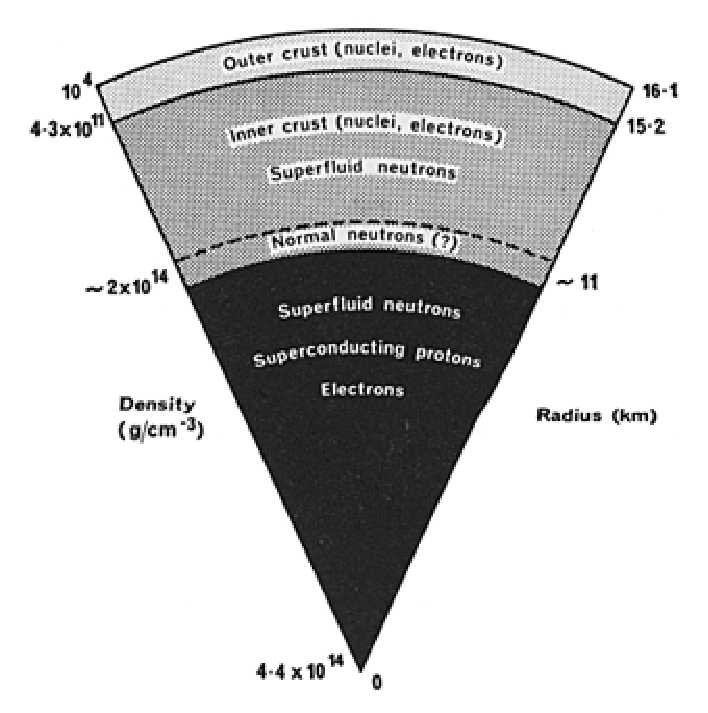
\includegraphics[height=90mm, width=120mm]{neutron_star_structure.eps}
	\caption{Hypothetical internal structure of a neutron star (Citation: \url{http://heasarc.gsfc.nasa.gov/docs/objects/binaries/neutron_star_structure.html})} 
        %CITE Possibly original Frank Shu? Fred would probably know, being a student of Frank
	\label{neutron_star_structure}
	\end{center}
	\end{figure}


Spinning neutron stars (NS)~\cite{Prix2006} motivate clear yet computationally-challenging GW searches.
Perhaps one NS is born per century in the Milky Way~\cite{NarayanOstriker1990}.
In the solar-system reference frame, isolated NS would emit a pure sine wave, as predicted by (with leading constant $G_C/c^4$) Equation~\ref{Fourier-domain-quadpole-eq}.
        The emission mechanism of gravitational radiation with amplitude $h_0$ from a NS is from an elliptical deformation, ellipticity $\epsilon$, on its surface (outer crust, Figure~\ref{neutron_star_structure}), leading to a quadrupole moment $I$~\cite{Zimmermann1979,LSCPulsar2006} and thus emission at frequency $f = 2\nu$, twice the NS spin frequency $\nu$:

        \begin{eqnarray}
        \epsilon &=& \frac{I_{xx} - I_{yy}}{I_{zz}}, \\
        h_0 &=& \frac{4 \pi^2 G_C}{c^4} \frac{I_{zz} f^2}{r} \epsilon.
        \end{eqnarray}

Ellipticity might arise due to $r$-mode oscillations, a deformation, or free precession~\cite{Shawhan2010}.
Expected sensitivities for terrestrial interferometers, best around 100 Hz, highlight NS with comparable periods (millisecond pulsars) as suggestive targets.
For GW from a rotating NS with a spin axis inclined at angle $\cos \iota$ to an observer's line-of-sight, the relative polarization amplitudes~\cite{DergachevThesis} would be,

\begin{eqnarray} 
h_+ &=& \tfrac{1}{2} h_0 (1 + \cos^2 \iota),\\
h_\times &=& h_0 \cos \iota.
\end{eqnarray}

For $\cos \iota = 1$, where the spin axis is along the line of sight, gravitational waves will thus be circular polarized; $\cos \iota = 0$, an orthogonally-aligned spin axis, implies linear polarization.
Excepting the case of torque balance~\cite{PapaloizouPringle1978,Wagoner1984} in low-mass X-ray binary systems (LMXB), NS rotation frequency will decay due to gravitational radiation, yielding a relationship between the `spindown age'~\cite{Brady1998} $\tau$ and the gravitational radiation amplitude:

        \begin{eqnarray}
        \tau &=& -f / \dot{f}, \\
        h_0 &=& \frac{1}{r} \sqrt{\frac{5 G_C I_{zz}}{2 c^2 \tau}}.
        \end{eqnarray}

%            Continuous -- specifically, binary neutron stars and rate predictions. Describe archetypical search methods as in the 1998 analysis paper~\cite{Jaranowski1998}, the Abbott et al paper~\cite{LSCPulsar2006}, including StackSlide~\cite{LSCPulsarS4}, Einstein at Home~\cite{LSCEinsteinHome2009}, and the most interesting to date from Michigan, Vladimir's PowerFlux~\cite{LSCPowerFlux2009}. Discuss earlier results from the earliest period~\cite{Abbott2004} and an early search for Scorpius X-1~\cite{AbbottPulsar2006}. Reinhard Prix is probably another good source~\cite{Prix2006}.
Although pure sine waves are considerably simpler than the numerical relativistic templates needed for inspirals, the low expected $h_0$ and consequent long-duration integration needed to detect NS mean that the search over parameter space is extremely sensitive to mismatched templates.
This sensitivity implies that the algorithms must use fine-grained templates, necessitating long computational time.
Algorithms developed from maximum likelihood estimates of isolated NS~\cite{Jaranowski1998}, incorporating progressively barycentric solar-system correction~\cite{LSCPulsarS4}, distributed computing~\cite{LSCEinsteinHome2009}, and semi-coherent methods~\cite{LSCPowerFlux2009}.
Many isolated pulsars~\cite{Abbott2004,LSCPulsar2006}, including the Crab and Vela pulsar remnants~\cite{AasiPulsarInitialResults2014}, as well as the LMXB Scorpius X-1~\cite{AbbottPulsar2006} and the direction of the the Galactic Center~\cite{AasiGalacticCenter2013} have been the target of these methods.

Many NS in known catalogs, such as ATNF (Australia Telescope National Facility~\cite{ManchesterATNF2005}), that pulsate in the LIGO frequency band are in binary systems.
This thesis develops, in Chapters~\ref{chap5} \& \ref{chap6} where this discussion continues, a computationally-efficient means, TwoSpect~\cite{GoetzTwoSpectMethods2011} of searching for NS in binary systems, particularly LMXBs. 
First, we discuss how gravitational wave interferometers sensitivity can be improved to make astronomy possible.

    \section{Laser Interferometer Gravitational-wave Observatories}
    \label{LIGO}
        
Design and construction of the Laser Interferometer Gravitational-wave Observatories required extensive prototyping and commissioning both during Initial LIGO~\cite{MavalvalaThesis,AdhikariThesis,BallmerThesis} and Enhanced LIGO~\cite{FrickeThesis,SmithThesis,DooleyThesis}.
The core features of interferometer design were established even before construction, summarized by Saulson~\cite{Saulson}, but many technical noise sources were encountered.
Motivations, fundamental noises, and the developments of commissioning all merit attention.

%        LIGO observatories. The most fun part to write. Cite Nergis Mavalvala~\cite{MavalvalaThesis}, Stefan Ballmer~\cite{BallmerThesis}, Rana Adhikari~\cite{AdhikariThesis}, Nicolas de Mateo Smith-Lefevbre~\cite{SmithThesis} and, of course, Peter Saulson~\cite{Saulson}.

        \subsection{From Weber bars to interferometry}
        \label{bars_to_interferometry}

Between the earliest interferometry of Michelson~\cite{michelson} and LIGO came the resonant bar detectors of Joseph Weber~\cite{Weber1960}.
Bar detection of GW developed rapidly through the 1960s, but contradictory results dampened enthusiasm~\cite{Saulson,CollinsGravityShadow}.
Nevertheless, great effort was devoted to technically-excellent bars such as ALLEGRO, AURIGA, EXPLORER, NAUTILUS and NIOBE over the subsequent decades.
Meanwhile, prototypes by Reiner Weiss, Robert Forward~\cite{Forward1978}, Ronald Drever and many others demonstrated that interferometry could also achieve the senstivities desired for gravitational wave detection.
Interferometry promised better fundamental noise sources and broadband operation, meaning that a single instrument could listen to a wider frequency band.
Xylophones of bars were proposed, but never built, that might scale the few Hz bandwidths of bars to the hundreds to thousands of Hz of interferometers.
Gravitational wave interferometry has carried the prospects for GW astronomy toward unprecedented levels of sensitivity, thanks to performance factors detailed in Section~\ref{methods}.

            %History lesson: Weber bars progress to interferometers. Use Saulson, but Nic's thesis has links to some of the original sources~\cite{Saulson},~\cite{SmithThesis}.           

        \subsection{Observatories, investigations, and enhancements}
        \label{methods}

	Michelson invented modern interferometry~\cite{michelson} in his 1887 experiments with Morley to try to measure the velocity of the Earth with respect to the lumineferous ether.
Although commonly claimed to have spurred the work of Minkowski, the implications of this work for special relativity may not have been fully understood for several decades~\cite{CollinsGravityGhost}.
Yet the value of the experimental technique was undeniable.
Michelson \& Morley had invented an accurate relative phase-meter for light.

Existing GW observatories, at their cores, are also Michelson interferometers. 
In contemporary GW interferometers, monochromatic laser light (typically 1064 nm) is used.
This light is split into two equal beams by the beam-splitter, reflects off mirrors at the ends of two arms, X and Y, and returns to interfere at the beam-splitter after times $T_x$ and $T_y$.
The power $P$ at the beam-splitter output `dark' port, is by design equal to zero except when the measureable (e.g., ether, a GW, or other disturbance) causes a fringe shift $\Delta \phi$ related to the angular frequency $\omega$ of the light and the time-of-flight down the $x$ and $y$ arms, $T_x$ and $T_y$. 
Energy is conserved; the change of sign on the beam-splitter reflective surface means that destructive interface on the `dark' port implies constructive interface on the opposite 'bright' port.
Power is classically proportional~\cite{JacksonEM} to the electric field~\cite{Saulson}:

\begin{eqnarray}
P &=& \frac{\epsilon_0 c E_0^2}{2} \left| 1 - e^{i \Delta \phi}\right|^2 = 2 \epsilon_0 c E_0^2 (1 - \cos \Delta {\phi}),
\label{michelson-interferometry-eq}\\
\Delta \phi &=& 2\pi (L_s + L_0) /\lambda + \omega (T_y - T_x).
\end{eqnarray}

In Enhanced and Advanced LIGO, $L_s$ is known as the Schnupp asymmetry (a constant difference in arm length related to RF-modulated sidebands)~\cite{AdhikariThesis}, and $L_0$ is a smaller constant offset from a fringe to enable non-radio-frequency-modulated DC readout~\cite{FrickeThesis}.
A putative, even smaller `DARM' phase shift can read out $\omega (T_y -T_x)$, due to differential arm motion, encoding any time-varying GW signal in the relative time-of-flight between the arms. 
Operating near the maximum of $dP/d(\Delta\phi)$ would increase susceptibility to unwanted power fluctuations, so the interferometer was initially operated with radio-frequency modulation at minimum $dP/d(\Delta\phi)$ and  $P$ (a dark fringe), later changed to a slight offset and DC readout once the noise sources were better understood.

Power $P$ can be directly improved by increasing effective laser power (e.g., a brighter laser or use of `power recycling'), and $\Delta \phi$ can be increased by making $T_{x,y}$ storage times longer (e.g., with Fabry-Perot cavities).
Doing so allows more accurate measurements of $P$ in the presence of shot noise (fluctuations in photon counting, entering via the $E_0$ term), radiation pressure (photon momentum-induced fluctuations in the mirrors causing changing in $T_y - T_x$), and other motions that change $\Delta \phi$ (such as thermal and seismic).
Yet these noise sources implicate quantum effects, and the photodiodes used to measure power do so with a certain quantum efficiency.
More realistic descriptions by Caves~\cite{Caves1980,Caves1981} clarify the quantum mechanical origin of shot and radiation pressure noise.
Quantum squeezing, the subject of Chapter~\ref{chap4}, can mimic the effect of higher power in Equation~\ref{michelson-interferometry-eq}.
GW, an eminently classical phenomenon, are small enough in amplitude that quantum behavior is a key limit on its detection.

Gravitational wave signals enter the interferometer by changing the spacetime curvature in the arms. 
In the simplest, linearized picture, the spacetime curvature arises from a GW with amplitude $h$ at frequency $f$.
When the GW is linearly polarizared in $h_+$ and aligned with x-axis and y-axis arms of equal length $L$ (see~\cite{Jaranowski1998} for the antenna pattern correction when it is misaligned), it changes the time-of-flight in the arms according to Equation~\ref{GW-matrix-eq}:

\begin{eqnarray}
T_x = \int_0^{\frac{2L_x}{c}} \sqrt{|g_{xx}|} dt \approx \int_0^{\frac{2L_x}{c}} \left(1 - \frac{h_+ (t,x(t))}{2} \right) dt, \\
T_y = \int_0^{\frac{2L_y}{c}} \sqrt{|g_{yy}|} dt \approx \int_0^{\frac{2L_y}{c}} \left(1 + \frac{h_+ (t, y(t))}{2} \right) dt,
\end{eqnarray}

\noindent We have been able to neglect issues of the proper-time of the mirrors (as opposed to the photodiode) because the laser frequency $\omega$ is unchanged ($g_{tt} = 0$ in transverse-traceless gauge).
The mismatch in the integrals leads to a detectable time-varying signal,

\begin{equation}
\phi_{\textup{DARM}} \equiv \omega (T_y - T_x) = \omega \int_0^{\frac{2L}{c}} \frac{h_+ (t, x(t)) + h_+ (t, y(t))}{2} dt.
\end{equation}  

\noindent Measured by Equation~\ref{michelson-interferometry-eq}, $\phi_{\textup{DARM}}$ encodes the GW signal.
Comparing $\phi_{\textup{DARM}}$ from different observatories, or waiting while a single observatory is Doppler-modulated by terrestrial motion, can pinpoint the origin of such a signal.

We often assume that the time-of-flight is much less than the GW period, $T_{x,y} \ll 1/f$.
This assumption is easily relaxed by accounting for the destructive self-interference of the signal light from a high $f$ signal~\cite{Saulson}.
A straightforward interpretation emerges for a quasi-static plane-wave (when phase offset $2\pi L_0/\lambda \gg \phi_\textup{DARM}$) -- the interferometer linearly transduces GW strain (via $h_+ = \phi_\textup{DARM}c/(2L\omega)$) into power:

\begin{eqnarray}
%h_+ &=& \frac{c}{2 L \omega}\phi_\textup{DARM},\\
\frac{d P}{d h_+} &=& \frac{2L\omega}{c}\frac{dP}{d(\Delta\phi)} = 4 L\omega \epsilon_0 E_0^2 \sin \left(\frac{2\pi}{c} (L_s+L_0) \right),\\
P &=& \left[ 4 L \omega \epsilon_0 E_0^2 \sin \left(\frac{2\pi}{c} (L_s+L_0) \right) \right] h_+.
\label{strain-to-power-eq}
\end{eqnarray}

% DONE:           Why GW interferometers work. Null measurements, a zeroed operating point. 
%The specifics are best handled by Saulson~\cite{Saulson}. 

%The idea of a Pound-Drever-Hall lock is most elegantly explained by Black~\cite{PDHNotes}. Rai Weiss may have some neat details, possibly historical, albeit that it is in a presentation~\cite{LIGOWorks}. The details of Fabry-Perot cavities in LIGO are handled by Rakhmanov, Savage et al~\cite{ResonanceFP},~\cite{ResponsesFP}. i

%DONE: The motivation for the evolution to Enhanced LIGO and its DC readout methods is covered well in the corresponding CQG article~\cite{Fricke2009} and specific details of its construction and operation are in Tobin Fricke's thesis~\cite{FrickeThesis}.

            \subsubsection{Interferometer theory in practice}
            \label{interferometer_theory}

Interferometers transduce GW strain into power in a manner like Equation~\ref{strain-to-power-eq} only because they operate in a linearly-controlled regime~\cite{FrickeThesis} with noise sources surpressed as well as possible~\cite{Saulson,LIGOWorks}.
A complete discussion of noise is beyond our scope, but the key limits on a ground-based GW interferometer arise, for a facility in vacuum, from microseisms, gravitational gradients, thermal coating and thermal suspension noise, and quantum effects (radiation pressure and shot noise).

Seismic noise is dominates the lowest frequences, and it is supressed by use of servo controls as well as passive damping from pendula.
Each stage of a multi-stage pendulum reduces, for frequencies above its natural resonant frequency $f_0$, the coupling of seismic noise into the interferometer by a factor $(f/f_0)^2$.

Gravitational gradients due to clouds, human activity, and density fluctuations in the ground are an area of concern, but may be addressed through active feedforward servos~\cite{Driggers2012ActiveNoise}, as may magnetic couplings.

Thermal coating noise is reduced by using larger laser spot sizes on the surfaces of mirrors and optimizing thematerial properties of the coatings; the mirror itself must be made of a material with a high $Q$, such as fused silica, where $Q$ is the quality factor for internal oscillations.
Suspension thermal noise is also reduced by using high $Q$ materials, per the fluctuation-dissapation theorem~\cite{Saulson}.
These effects predominate in the middle of LIGO's frequency range, often termed the `bucket'.

Shot noise is naively reduced by increasing laser power, which indeed yields improvements to a point.
At high laser power, however, thermal distortions due to absorption in the mirrors are inevitable, leading to the need for thermal compensation systems~\cite{BallmerThesis}.
High laser power also buffets the mirrors with radiation pressure noise, requiring heavier mirrors.
Quantum squeezing can circumvent the issue of thermal distortions, but it too induces radiation pressure noise (typically worse, because the Heisenberg uncertainty area increases); a solution may be squeezing at high (shot noise-limited) frequencies and anti-squeezing at low (radiation pressure-limited) frequencies.

%Noise sources dominate the 
%                GW interferometry theory: differential arm motion, key noise sources. 
%The main sources Saulson~\cite{Saulson} and Weiss~\cite{LIGOWorks}.
%                Here we discuss the key noises sources: seismic noise, thermal noise, and quantum (radiation pressure, shot noise).

GW interferometers on Earth are limited in size (thus storage time and strain sensitivity) by the planet's curvature (which couples vertical displacement noise into horizontal) as well as finances. 
GEO600 uses delay lines and the other interferometers use Fabry-Perot arms to extend the storage time of light.
Fabry-Perot arms with high-finesse~\cite{ResonanceFP,ResponsesFP} (roughly $137$ in Initial LIGO) are locked~\cite{PDHNotes} using the Pound-Drever-Hall (PDH) technique.
Elucidated below, electro-optic modulations (EOMs) provide a radio-frequency error signal for PDH locking the Fabry-Perot arms.

Figure~\ref{primary_eLIGO_optics} presents a schematic overview of the key systems in Enhanced LIGO.

\begin{figure}
\begin{center}
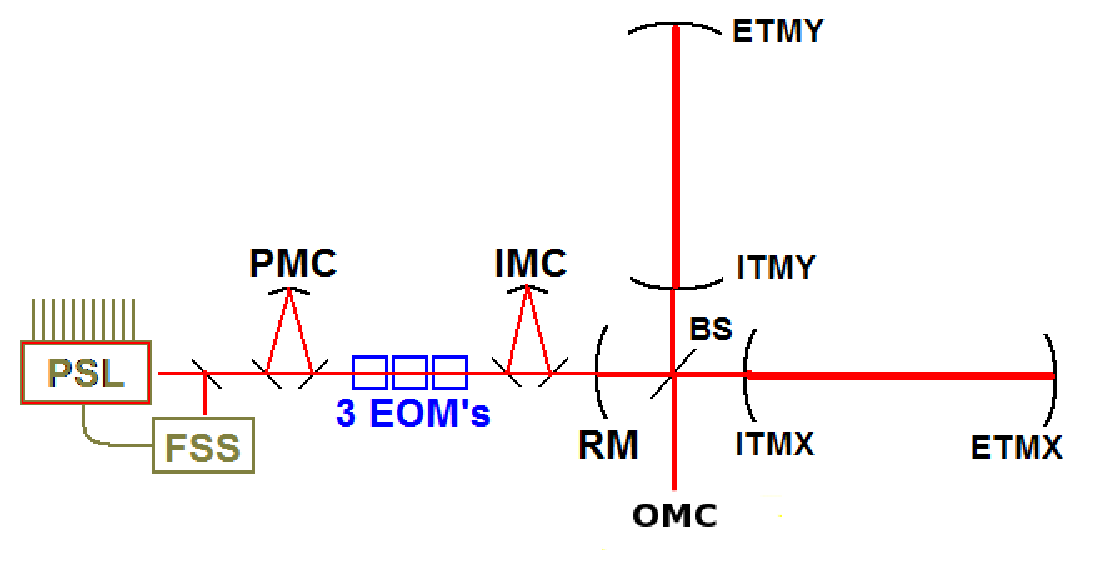
\includegraphics[height=90mm,width=148mm]{LIGODiagramnew.eps}
\caption{Enhanced LIGO primary systems and optics. From left, the phase-stablized laser (PSL) produces coherent light, kept at constant frequency by the frequency-stabilization servo (FSS). The pre-mode cleaner excludes non-Gaussian beamshapes, allowing only the $TEM_{00}$ mode to pass. The beam is the phase-modulated using three electro-optical modulators (EOMs) before being further shaped in the input mode cleaner (IMC). The beam passes through the power recycling mirror (RM) and is split at the beam-splitter (BS). Along the $X$ and $Y$ arms, light resonates in the Fabry-Perot cavity formed between the input test mass (ITM) mirror and the end test (mass) ETM mirror, before recombining at the beamsplitting. Any light with the same phase as before the arms is returned to the interferometer by the RM, but if phase-shifted, perhaps by a gravitational wave, it exits through the output mode cleaner (OMC): a photodiode just downstream of the OMC records the signal.}
\label{primary_eLIGO_optics}
\end{center}
\end{figure}

            \subsubsection{Observatory operation}
            \label{observatory_operation}

	\begin{figure}
	\begin{center}
	\includegraphics[height=111mm, width=148mm]{Screen_shot_2010-07-21_at_042516.eps}
	\caption{Screenshot of MEDM control panel. MEDM is a Motif Epic and Display Manager for EPICS, the Experimental Physics and Industrial Control System, which lets operators control LIGO. MEDM allows operators to run locking scripts as well as alignments and tests, and to activate and de-activate filters.}
	\label{ScreenshotMEDM}
	\end{center}
	\end{figure}

Satisfying the noise requirements above, the first-generation LIGO interferometer was designed with the following features:

\begin{itemize}
\item Power recycled Michelson interferometer with 4 km Fabry-Perot arms\footnote{A second 2 km interferometer was sited at Hanford as well during Initial LIGO.}
\item Hanford, Washington and Livington, Louisiana observatories
\item 4 km perpendicular beam tubes
\item $10^{−9}$ torr vacuum
\item 10 W Nd:YAG 1064 nm laser (Enhanced LIGO upgraded to 20 W)
\item 10 kg fused silica primary optics
\item 4-stage seismic isolation (including active hydraulics at Livingston)
\item Laser frequency stabilization
\item Angular sensing and control (wavefront sensors, optical levers)
\item Length sensing and control (magnet coils, common mode)
\item Pre- \& input-mode cleaning (Enhanced LIGO added output mode cleaning)
\item Power recycling
\item Digitally filtered servos and readout
\item RF heterodyne (Initial LIGO) or DC homodyne (Enhanced LIGO) readout
\end{itemize}

LIGO's digital systems were managed with MEDM and EPICS, seen in Figure~\ref{ScreenshotMEDM}.
Extensive effort on installation was required to attain the necessary angular, length, and auxiliary servo control needed for Initial LIGO operation~\cite{ReadoutGWA}.
Once at design sensitivity, S5 succeeded in obtaining the desired sensitivity and duty cycle.
Although the RF heterodyne technique\footnote{Curiously, the RF sidebands were not always equal in the recycling cavity~\cite{MeadorsHanford2005}.} had good low-frequency sensitivity, it limited the shot noise performance compared to a DC homodyne instrument by a factor of $\sqrt{3/2}$, and squeezing was also easier in DC.
The switch to DC readout occured prior to S6, and in the leadup to that science run, substantial detector characterization was needed to understand the upgraded interferometer.

%                Operating LIGO: controls, Detector Characterization. One of the first sources from initial LIGO to read up on is a paper by Fritscel, Bork, Mavalvala et al~\cite{ReadoutGWA}. Initially this system made a detection based on heterodyne readout using GW sidebands, which, among other troubles, could be unequal in the recycling cavity~\cite{MeadorsHanford2005}.


                \paragraph{Detector characterization}
                \label{detchar}
            
%                    DetChar methods: omega scans, line hunting and glitches

\begin{figure}
\begin{center}
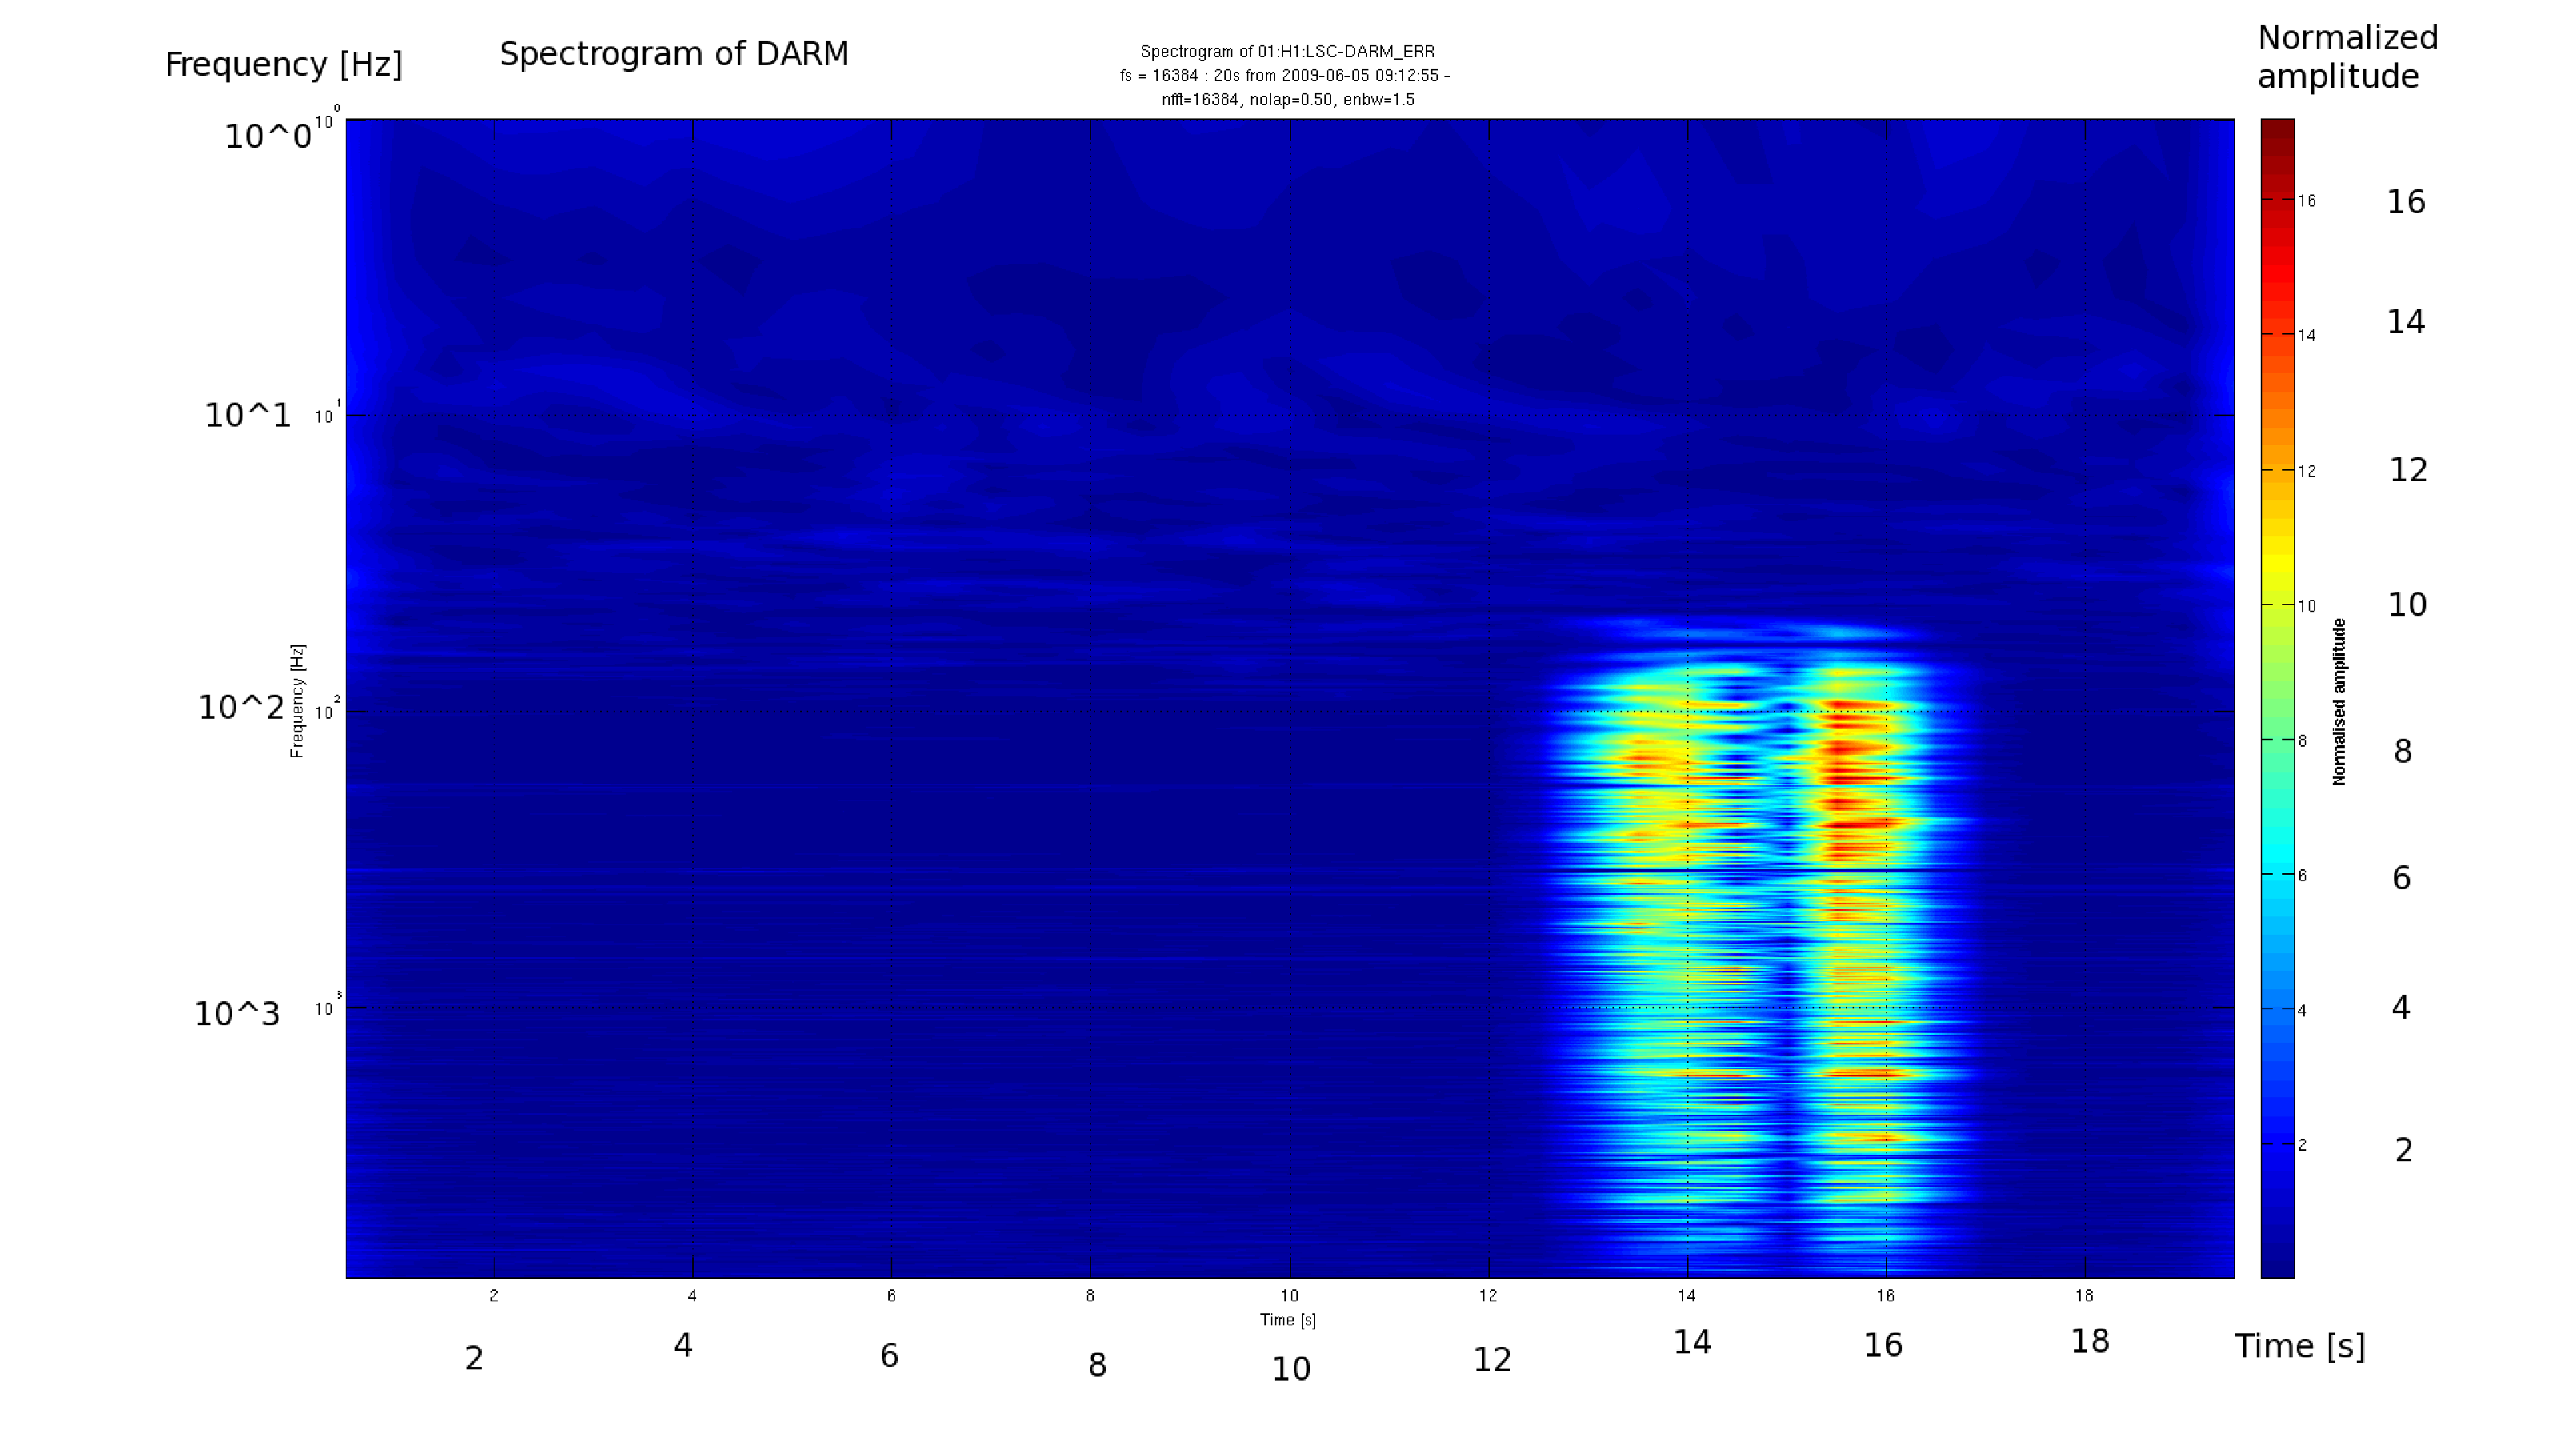
\includegraphics[height=111mm, width=148mm]{aglitch928228390_new.eps} 
\caption{Omega scan of an audible broadband glitch. Shortly before the start of Science Run 6, detector characterization took place to identify categories of glitches, such as the `gremlin', and to eliminate them. The burst group analysis pipeline, Omega, generated time-frequency spectrograms that made this identification easier. Glitches are a limiting factor in the identification of rare events and therefore of potential gravitational wave burst signals.}
\label{omega_scan_audible_glitch}
\end{center}
\end{figure}

Commissioning Enhanced LIGO in the three months encompassing the start of S6 around July 2009 required eliminating the residual noise sources lingering from installation. 
In particular, the Output Mode Cleaner~\cite{SmithThesis} was an unknown, and its servo-locking scheme (involving both piezoelectric and thermal actuation) required some artistry.
DC readout generally increased the low-frequency noise floor.
New glitches sprang forth as a results, and the author's work at LIGO Hanford Observatory centered on identifying them.

Common tools for investigators on-site are both time-domain (DataViewer) and frequency-domain (Diagnostic Test Tools) data-plotters.
While those perspectives allowed diagnosis of at least one flaw in the interferometer's filters, a combined, spectrogrammatic view using the burst group's Omega analysis pipeline proved a needed third, unified view, seen in Figure~\ref{omega_scan_audible_glitch}.
This pipeline was run on many pre- and early-S6 glitches using a manual infrastructure\footnote{Omega scan diagnostics were later automated by Tomoki Isogai.}.

Effective engines for tracking and, preferably, eliminating glitches and persistent lines in the detector spectrum -- the process of detector characterization -- are critical to distinguishing rare events.

%My work on site included getting the Omega scan engine tested and running manual Omega scans in the first months of S6, July and August 2009. 
%See Figure~\ref{omega_scan_audible_glitch} for an example of the spectrograms this method was able to generate. These spectrograms helped categorize glitch sources and reduce them, to the benefit of the burst group in particular.
%Fortunately, this work was later automated thanks to Tomoki Isogai. 

                \paragraph{Feedforward filtering}
                \label{feedforward_filters}

Feedback servos keep LIGO operational, holding the mirrors and auxiliary systems in stationary `lock' points.
Closing the loop in feedback requires a way to actuate a physical control signal to cancel out whatever influence is causing an error signal that pushes the system away from its lock point.
When this direct cancellation is not possible -- for instance, when ambient magnetic fields due to 60 Hz mains lines can not be escaped -- feedforward remains.
Feedforward, an open-loop, can be done purely in software, but it requires an accurate estimator for the influence of a noise source into the system.

In the case of Enhanced LIGO commission, an example was implemented with the aforementioned 60 Hz line using a magnetomer to supply the feedforward correction~\cite{SmithThesis}, which greatly enhanced sensitivity near the Crab pulsar frequency.
Subsequently, into the following years, I began to work on the long-known~\cite{AdhikariThesis,BallmerThesis} issue of cancelling the influence of auxiliary length control noises.
Loops for nulling this effect exist, diagrammed in Figure~\ref{servo_loop_realtime}, but they require periodic retuning~\cite{KissellPRCMICH}.  
The direction of this work was to fine an automated, and more precise, way to tune these servos.
A finely-tuned servo filter was implemented in late September 2010\footnote{After, and unrelated to, the famed Big Dog event~\cite{Riles2013}}.
This filter reduced the noisiest residual coupling, from the differential inner Fabry-Perot mirror motion to the differential arm motion that encodes strain, by almost an order of magnitude. 

                    %Example of feedforward: 60 Hz magnetometer. The only source that mentions this is, I think, Nic's thesis~\cite{SmithThesis}. Yet the most pertinent example is one that has long been applied to LIGO: MICH and PRC feedforward. The specific needed are mention in the thesis of Adhikari~\cite{AdhikariThesis} and Ballmer~\cite{BallmerThesis}, but immediately before Keita Kawabe and I began our project, these parameters had been tuned by Jeff Kissel~\cite{KissellPRCMICH}

	\begin{figure}
	\begin{center}
	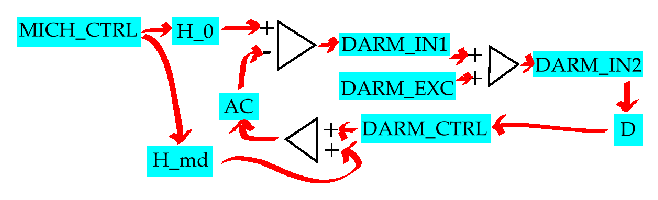
\includegraphics[height=80mm, width=148mm]{servo_loop.eps}
	\caption{Real-time servo loop diagram. The MICH\_CTRL signal can be though to leak into the true DARM signal via a transfer function, H\_0. (The letter `h' is typical for transfer functions as well as gravitational wave strain; coincidentally, this is a noise transfer into the channel for displacement, DARM, which is proportional to strain $h(t)$). H\_0 leaks into error signal, which is otherwise kept null thanks to the servo cancellation provided by DARM\_CTRL times a physical actuation function AC. The measured error signal is DARM\_IN1. If desired, an excitation can be supplied via DARM\_EXC for a sum of DARM\_IN2. This error signal passes though digital filters D to yield the aforementioned control signal DARM\_CTRL. The auxiliary length cancellation loop is simply adding H\_md to DARM\_CTRL in order to subtract out the corruption of H\_0.}
	\label{servo_loop_realtime}
	\end{center}
	\end{figure}

	\begin{figure}
	\begin{center}
	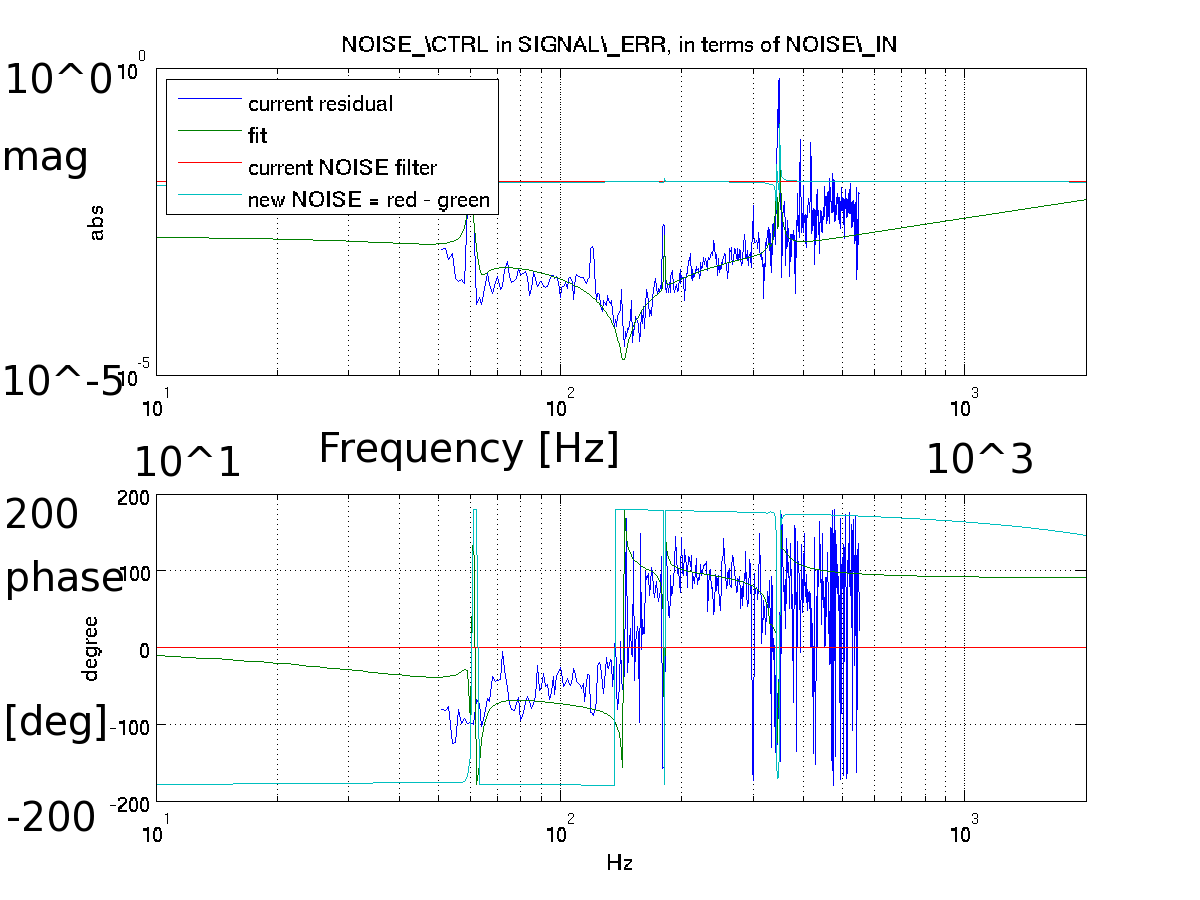
\includegraphics[height=111mm, width=148mm]{newNOISEfilter.eps}
	\caption{Real-time work on a LIGO noise filter. This Bode plot, made in Matlab, shows the correction to the existing MICH damping (cancellation) loop needed mid-2010, toward the end of Science Run 6. The correction is small, because the majority of the coupling fits the flat model expected from theory. This transfer function estimate suffices for post-factor correction. However, in order to be incorporated into the control scheme shown in Figure~\ref{servo_loop_realtime}, measurements of the open loop gain $G$ and actuation function AC are necessary to yield incorporate the filter correctly into the closed loop response.} 
	\label{newNOISEfilter}
	\end{center}
	\end{figure}

The closed loop gain mentioned in Figure~\ref{newNOISEfilter} is a function of frequency because it is a geometric sum of time $\tau$-delayed open loop gain responses by DARM\_CTRL to error signals from DARM\_ERR: $G_\textup{closed} = \lim_{p\rightarrow\infty} \Sigma_n^p G e^{i n \omega \tau} = \left(1 + G e^{i \omega \tau} \right)^{-1}$. 
Because MICH damping is summed with DARM\_CTRL, it picks up an additional factor of the actuation function AC for a net transfer function of $H_{md} G_\textup{closed}$AC in the closed loop. 
Thus, compared to an open-loop (e.g., post-facto) subtraction (effect estimated in Figure~\ref{filter_early}), a real-time servo will differ by a factor of $G_\textup{closed}$AC. 
See Chapter~\ref{chap3} for full details of open-loop subtraction and the extension to a post-facto, veto-safeguarded improvement in the sensitivity of all S6.

	\begin{figure}
	\begin{center}
	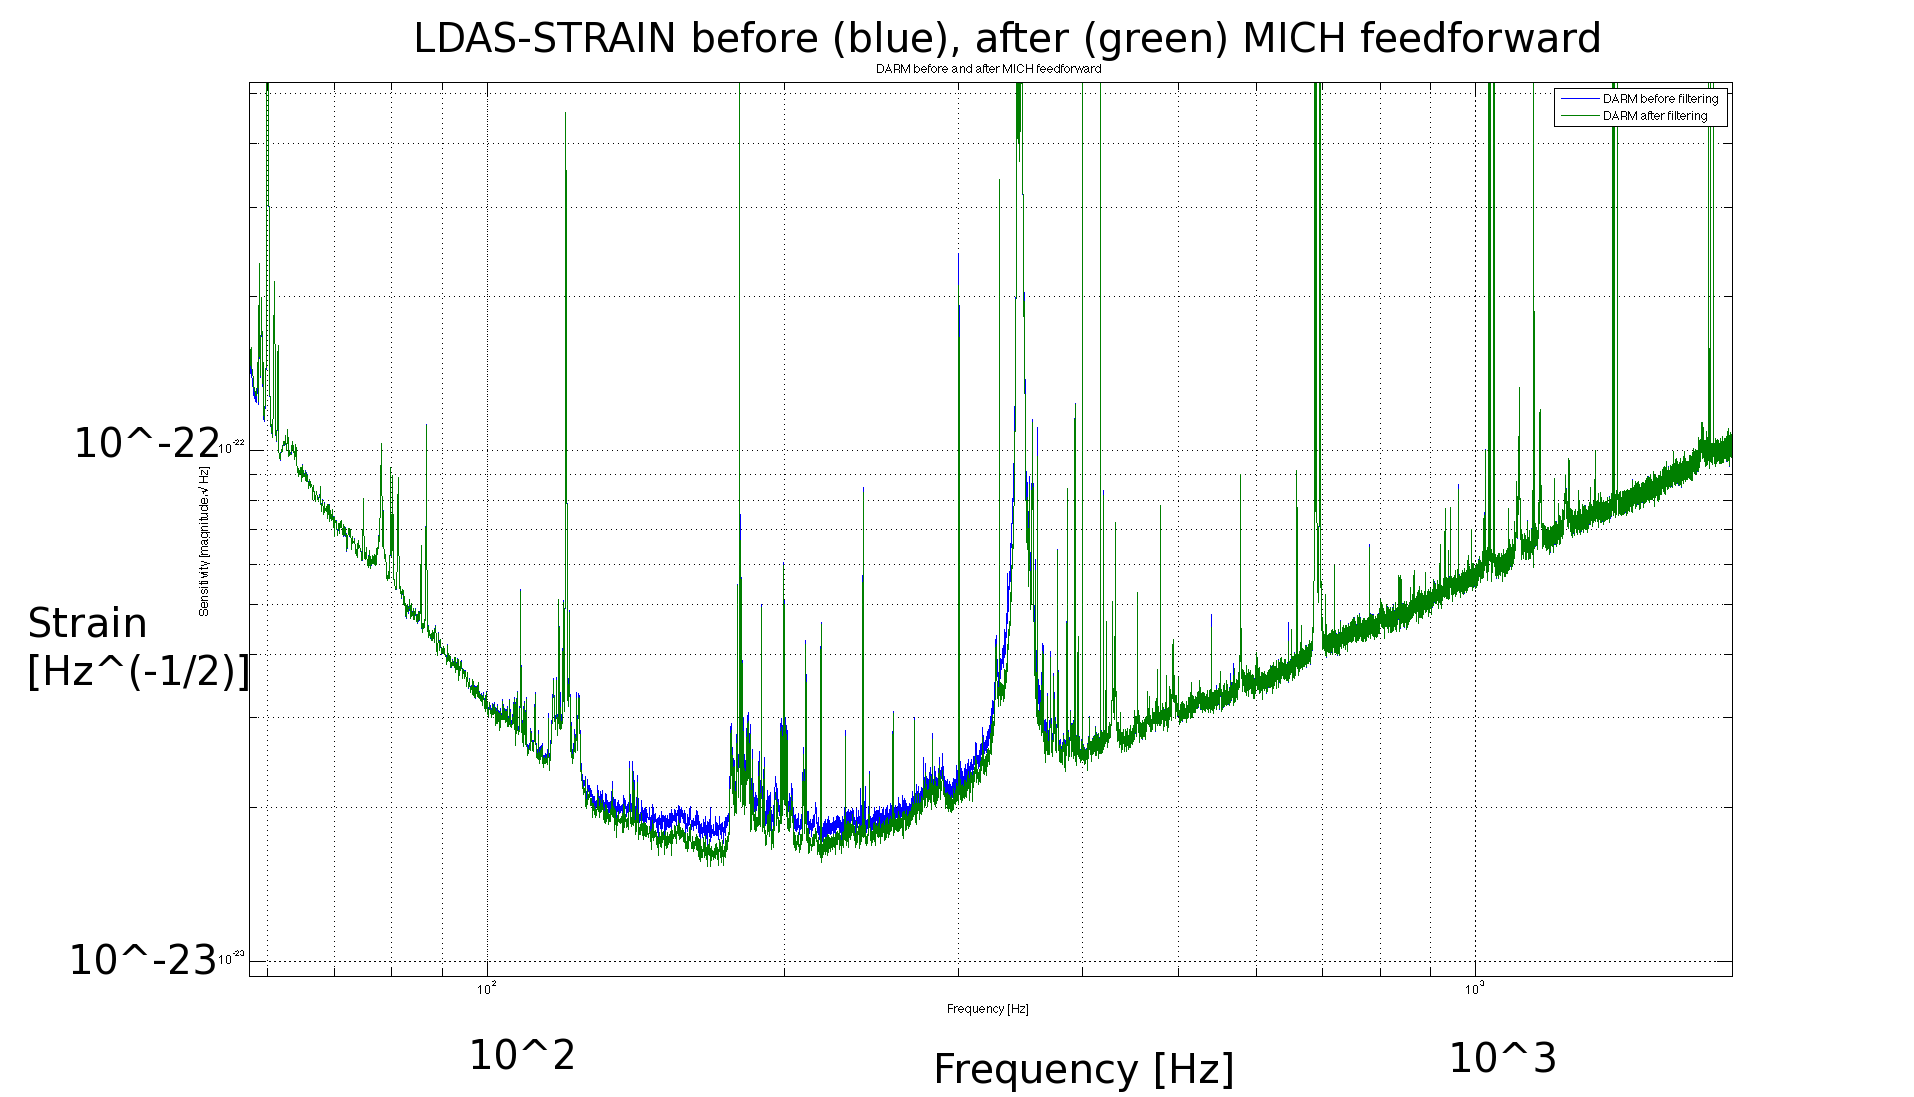
\includegraphics[height=90mm, width=148mm]{2011-03-08_filter-01.eps}
	\caption{Early work on post-facto noise filtering. After testing out MICH damping filters offline, post-facto, the correction factors for AC and $G_\textup{closed}$ were incorporated and the entire filter imported using Foton into the EPICS control system, where it was used real-time from the September equinox of 2010 until the end of Science Run 6.}
	\label{filter_early}
	\end{center}
	\end{figure}

                \paragraph{Phase camera}
                \label{phase_camera}

Improving length control is intuitive, since length directly correlates with LIGO's inference of GW strain.
Angular control, however, is just as necessary: LIGO uses quadrature-photodiode wave-front sensors~\cite{MavalvalaThesis} to minimize misalignment.
Misalignment causes direct angle-to-length coupling, adding noise to the system by corrupting the phase measurement at readout; it also permits power fluctuations in the Fabry-Perot arms, reducing shot noise-limited performance and, when the relative power returning from the arms (the contrast defect) changes, directly corrupting the power measurement at readout~\cite{DooleyThesis}.
Therefore more sophisticated systems have been researched in hopes of reducing angular fluctuations still further, culminating in the phase camera at Michigan~\cite{DergachevThesis}.

%                    Future devices: overview of phase camera with Vladimir. Vladimir's thesis definitely talks about it~\cite{DergachevThesis}. We can discuss the fundamentals behind the need for angular stabilization and control from Nergis Mavalvala's thesis~\cite{MavalvalaThesis}, but we can refresh it with a modern reference from Kate Dooley's thesis~\cite{DooleyThesis}.
\begin{figure}
\begin{center}
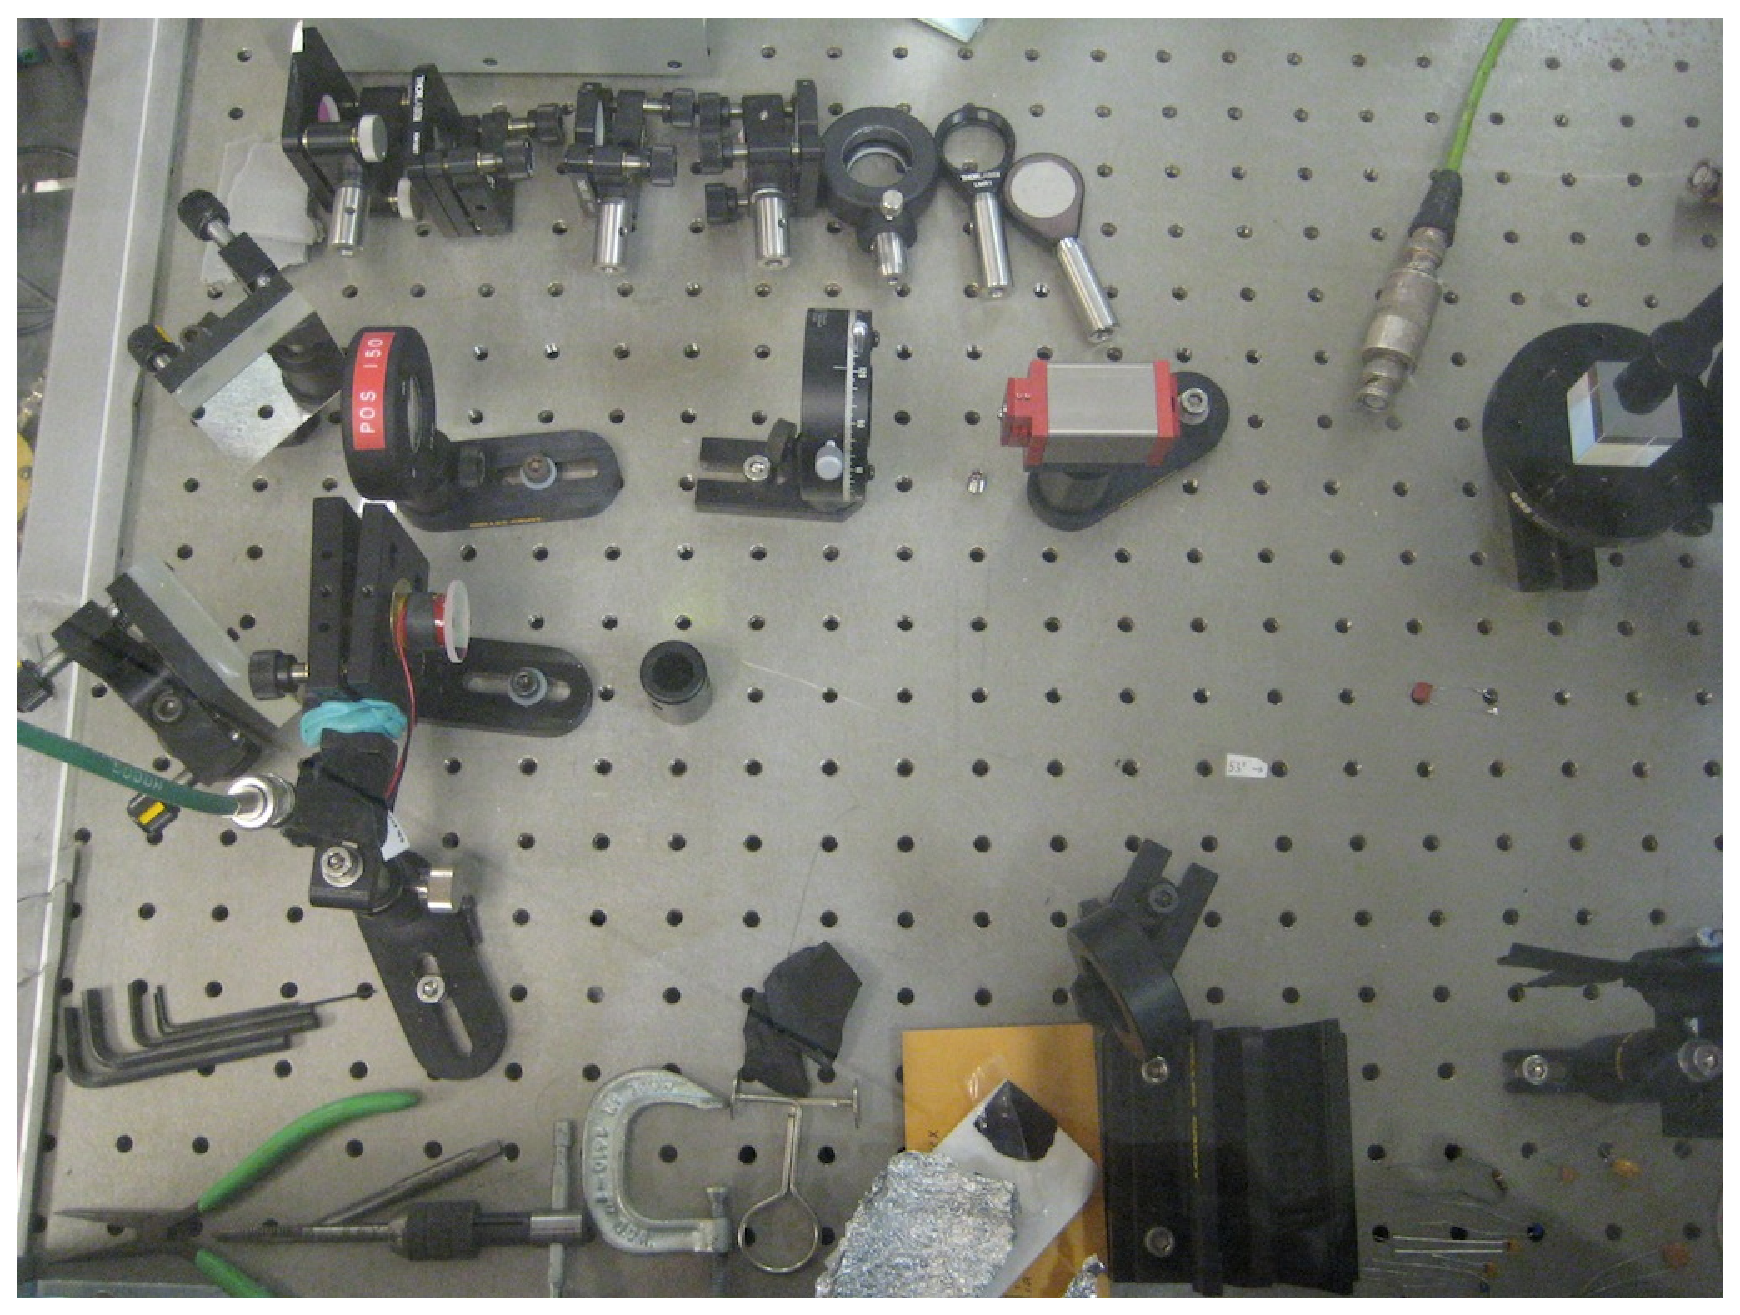
\includegraphics[height=111mm, width=148mm]{Optical_table_phase_camera.eps}
\caption{Optical table layout with Fabry-Perot cavity and Pound-Drever-Hall locking for phase camera. Faraday isolator and polarizing beam-splitter at upper right; piezoelectrically-actuated mirror at center left. Difficulties with stability, despite a plexiglass enclosure and floated table, meant that locks were fractions of a second at most, hampering efforts.}
\label{phase_camera_optical_table}
\end{center}
\end{figure}

Locking used the Pound-Drever-Hall (PDH) method~\cite{PDHNotes,MavalvalaThesis}.
Mathematically, the method assumes two mirrors: an input, with amplitude reflectivity $r_1$, and an end, with amplitude reflectivity $r_2$.
Upon the input mirror is incident a coherent electric field, due to light, $E_\textup{inc}$ at frequency $\omega_0$. A field $E_{\textup{refl}}$ is reflected.
The key to the technique is that the incident electric field is phase modulated by a factor $\Gamma$ with modulation frequency $\Omega$, by a device such as an electro-optic modulator (EOM, e.g., a Pockels cell).
Typically this modulation is done at radio-frequency.
This EOM modulates an electric field of amplitude $E_0$ into higher and lower frequency sidebands, amplitude $E_+$ and $E_-$, as determined by expansion in Bessel functions $J_n(\Gamma)$ -- higher order sidebands exist at usually-negligible amplitude.
From the reflected signal, then, the intensity $I$ encodes an error signal of the arm length $l$, for given light wavenumber $k = \omega / c$, at the modulation frequency (aside from additional signals at DC and at 2$f$):

\begin{eqnarray}
E_{\textup{refl}} &=& \frac{r_1 - r_2 e^{-2 i k l}}{1 - r_1 r_2 e^{-2 i k l}} E_\textup{inc},\\
E_\textup{inc} &=& E_0 e^{i \Gamma \cos \left( \Omega t \right)} \approx E_0 e^{i \omega_0 t} \left[ J_0 (\Gamma) + J_1 (\Gamma) e^{i\Omega t} + J_{-1} (\Gamma) e^{-i \Omega t} \right],\\
E_\textup{refl} &\approx& e^{i \omega_0 t} \left[ E_0^\textup{refl} + E_+^\textup{refl} e^{i\Omega t} + E_-^\textup{refl} e^{-i \Omega t}\right],
\end{eqnarray}
\begin{equation}
\begin{split}
I =& \left[ |E_0|^2 + |E_+|^2 + |E_-|^2\right] + \\ 
  & \left[(E_0^* E_+ + E_0 E^+_-)e^{i\Omega t} +\textup{C.C.} \right] + \\
  &\left[E_+ E_-^* e^{2i\Omega t} +\textup{C.C.} \right].
\end{split}
\end{equation}

Radio-frequency photodiodes are generally needed to record this intensity with its modulation.
Typically, the photodiode current is demodulated with a mixer that uses as local oscillator the same sine wave that drives the Pockels cell EOM phase modulation.
Alternative photoresistor readouts were explored in hopes that they might have faster response times since the standard electronics references were compiled~\cite{HorowitzHill1989,Simpson}, because of their potential desireability for a many-pixel readout.
%The electronics development were guided by Horowitz and Hill~\cite{HorowitzHill1989} as well as by Simpson~\cite{Simpson}.
Using the usual RF photodiode, a Fabry-Perot cavity was built prior to this author's work~\ref{phase_camera_optical_table}.
Numerous attempts to stabilize the cavity and derive a useful PDH locking signal were made, the laser was upgraded, EOM replaced, and the analog locking system frequency response was characterized.
Unfortunately, locks proved too fleeting to pursue a program of intentional mis-alignment and correction based the phase camera angular measurements.
Much progress nonetheless was made by Dergachev in realizing effective methods of high-speed digitization of the RF-modulated signal in free space~\cite{DergachevThesis}.
%See Figure~\ref{phase_camera_optical_table} for a picture of the cavity as built.


        \subsection{Advanced observatories and beyond}
        \label{advanced}
  
            %Advanced LIGO and beyond -- squeezing and prospects?
%DUSEL, 
	Advanced LIGO~\cite{aLIGOrefDesign,aLIGOsysDesign} is intended to improve upon the first-generation LIGO inspiral range tenfold, to 200 Mpc.
To accomplish this, it simultaneously must lower the noise floor at the most sensitive frequencies, to a strainnoise  $4\times10^{-24}/\sqrt{\textup{Hz}}$, and push the low-frequency wall of seismic noise down, so that frequencies as low as 10 Hz (rather than about 50 Hz) could be probed.
While maintained in the same vacuum envelope, the optical systems are far superior.
The 10 kg fused silica test mass mirrors have been upgraded to 40 kg for better radiation pressure performance.
Fused silica fibers with high $Q$ suspend the mirrors, instead of steel piano wire; fibers are welded directly to the test mass.
Rather than a single pendulum, each test mass sits at the bottom of a four-stage `quad' actively-servoed pendulum chain, reducing seismic noise by a factor of $(f/f_0)^8$.
The quad pendulum itself is attached to a new in-vacuum seismic isolation table (similar tables hold the auxiliary optics).
These test masses indeed need to be heavier.
Laser power has increased from 20 W in Enhanced LIGO to 200 W in Advanced LIGO.
Fabry-Perot arm cavity finesse has also increased, raising the stored arm power.
The arm cavities can be locked independently of each other and brought into the Michelson interferometer gradually, which should improve ease of use, quickly recover from lock-losses, and thereby improve reliable duty cycle, coupled with other system-wide improvements in control architecture.
Resonant sideband extraction is one of the most inventive changes, adding an additional signal recycling mirror to the optical configuration, which allows tuning the cavity pole of the Fabry-Perot arms and trading between different levels of high- and- medium-frequency shot noise-limited performance.

Although not part of the reference design, the success of the LIGO Hanford squeezing experiment~\cite{BarsottiNatureSqueezing,ChuaBackscatteredLight,DwyerPhaseNoise} noted in Chapter~\ref{chap4} make quantum optics a likely feature of any enhanced follow-up.

Once commissioned, Advanced LIGO's second-generation design should make possible detections at the rate of 40 per year~\cite{AbadieRates2010}. 
Hanford and Livingston have both upgraded their 4 km interferometers and are entering commissioning.
The 2 km Hanford interferometer had been intended to be upgraded, but its optics have found a new and likely more useful propect -- part of the growing network of observatories described in Section~\ref{worldwide}.

        \subsection{Worldwide network}
        \label{worldwide}
 
Gravitational wave signals are an unknown in astronomy.
It has long been recognized that multiple observatories with independent confirmation of a signal would be more persuasive evidence of detection than an isolated site.
Yet even once the field is established, additional observatories will permit better science.
Sky localization of inspiral and burst sources relies on relative arrival times of a GW signal~\cite{Saulson}.
Multiple, widely-seperate observatories give the best baseline.
Moreover, the data for continuous wave searches from seperate sites can often be coherently combined to yield a quieter noise spectrum.
LIGO is fortunate thus not to be alone in the pursuit of gravitational wave astronomy.

The second, 2 km Hanford interferometer will likely not be upgraded to Advanced LIGO.
            %Allies: 
Instead, its optics will form the core of the nascent LIGO India project~\cite{IyerIndia2011}, which will dramatically improve the accuracy of sky position measurements for gravitational wave transients.
In Japan, KAGRA~\cite{Kuroda2010} is being built; when completed with sapphire mirrors and cryogenic systems, it should reach comparable sensitivity to the LIGO interferometers.
Advanced VIRGO~\cite{Acernese2009} benefits from the first-generation superattentuator's superb seismic isolation performance; from it will be suspended new optics that reflect a more powerful beam.
Together, these second-generation ground-based interferometers should suffice to make direct detection of gravitational waves a reality.

Around the same time as these observatories make first detection, an entirely different technique of GW astronomy, pulsar timing~\cite{Hobbs2010}, may open up vastly lower frequencies ($\mathcal{O}(10^{-9})$ Hz).
The two techniques should prove complementary information about the gravitational sky, as distinctive as gamma ray telescopes are from radio.

Yet GW astronomy would become a true precision science if a third generation of instruments followed.
Third-generation interferometry could take place underground, either in proposed American DUSEL or the European Einstein Telescope~\cite{Punturo2010}, potentially with xylophone interferometers tuned to optimize sensitivity in different frequency bands.
Prospects in space appear even grander in the long-term, despite short-term setbacks. 
Following NASA withdrawal from the Laser Interferometer Space Antenna, LISA, in 2011, the European Space Agency has made a concerted push to launch LISA Pathfinder in 2015, with plans for a somewhat-reduced yet very capable eLISA in coming decades~\cite{Vitale2014}.
If eLISA launches, it may open the way for detect measurements of the most elusive gravitational signature: the background of the universe itself.
Both the DeciHertz Gravitational Observatory (DECIGO)~\cite{Ando2010} and Big Bang Observer (BBO)~\cite{Harry2006} proposals could, by midcentury, open up a vision of the cosmos in its earliest days.
%LISA Pathfinder to launch in 2015 and eLISA to follolw~\cite{Vitale2014}

    \section{Summary}
    \label{intro_summary}
 
        %Summary: strong motivation and instruments, need to find evidence of GW.    

Initial LIGO, during the science run S6, would have been able to see the coalescence of two neutrons stars at about twenty Megaparsecs, out in the Virgo cluster of galaxies, from sixty-five million years ago, when dinosaurs still walked the Earth. 
In the first week of Advanced LIGO lock at Livingston, following Memorial Day 2014, Advanced LIGO had a temporal range extending only as far back as when early humans began their diaspora from Africa -- a terrestrial parallel to the expansion of the cosmos.
When completed, the Hanford and Livingston second-generation interferometers should see back ten times beyond what S6 could, six hundred and fiften million years, to before the Cambrian explosion of life.
Perhaps in the third or fourth generation of interferometers, our view of the gravitational sky may stretch back to the age of the observable universe.
Even then, we will not have seen all that can be seen.
With the two long-range forces of the universe, electromagnetism and gravitation, giving two complementary views of spacetime, we still must build great machines to explore the sights they show, we must understand what we are seeing, and we must propagate that understanding. 

This thesis is a prelude to those efforts, from the building of the quantum optical squeezer, and the feedforward regression and continuous waves binary search, to our public interferometer exhibitions.   
Feedforward regression provides a microcosm of the complexities of gravitational wave interferometry, so there we will begin.


            
%        --------------------
%
%	Here is a sample chapter file. The chapters of the thesis
%	should be saved to seperate files such as
%	\textit{chapter1.tex}. In the file \textit{thesis.tex} the
%	\textit{input} command then includes these chapters into the
%	thesis. Note that none of the chapter files need any headers.
%	This header for each of these files is contained in
%	\textit{thesis.tex}. The file \textit{thesis.tex} also
%	includes the numbers system for the sections, figures,
%	theorems lemmas etc...

%\section{Sample Section}
%\label{sample_section}
%
%	This is what a sample section looks like. Let's conclude this
%	section with a sample theorem statement and proof.
%
%	\begin{theorem}
%	\label{sample_theorem}
%	The are an infinite number of prime numbers
%	\end{theorem}
%
%	\emph{Proof:} On the contrary assume there are a finite number
%	of primes $P_1, P_2, ... P_n$. Consider $\mathcal{P} = P_1 P_2
%	\cdots P_n+1$. $\mathcal{P}$ is not divisible by any of the
%	primes in our finite set. (Contradiction) $\square$
  

